\documentclass{beamer}
\usetheme{metropolis}           % Use metropolis theme
\metroset{numbering=fraction}
\usepackage{tikz}
\usetikzlibrary{arrows,positioning,shapes.geometric}
\usepackage{float}
\usepackage{makecell}
\usepackage{fancyvrb}
\usepackage[export]{adjustbox}
\usepackage{caption}
\title{Lecture 1.2 \\ Engineering Design with Embedded Systems}
\date{\today}
\author{Patrick Lam \\ Jeff Zarnett \\ Michael Giannikouris}
\institute{Department of Electrical and Computer Engineering}
\setbeamertemplate{caption}{\raggedright\insertcaption\par}
\setbeamersize{text margin left=12pt,text margin right=12pt}
\newcommand{\putat}[3]{\begin{picture}(0,0)(0,0)\put(#1,#2){#3}\end{picture}} % just a shorthand

\begin{document}
\maketitle

\section{Introduction to Embedded Systems}
	
	%Definition
	\begin{frame}{Definition}

		\begin{center}
			\begin{quote}
				A general-purpose definition of embedded systems is that they are
				devices used to control, monitor or assist the operation of equipment,
				machinery or plant. “Embedded” reflects the fact that they are an
				integral part of the system. In many cases, their “embeddedness” may
				be such that their presence is far from obvious to the casual observer.
				Even the more technically skilled might need to examine the operation
				of a piece of equipment for some time before being able to conclude
				that an embedded control system was involved in its functioning.
			\end{quote}
		\end{center}
		
		\begin{flushright}			
			(Institute of Electrical Engineers)
		\end{flushright}	
		
	\end{frame}  
	
	\begin{frame}{Where Can You Find Embedded Systems?}
		\begin{tabular}{c c c c}		
			
\includegraphics[width=6em]{img/phone-icon-android-phone.png} &
			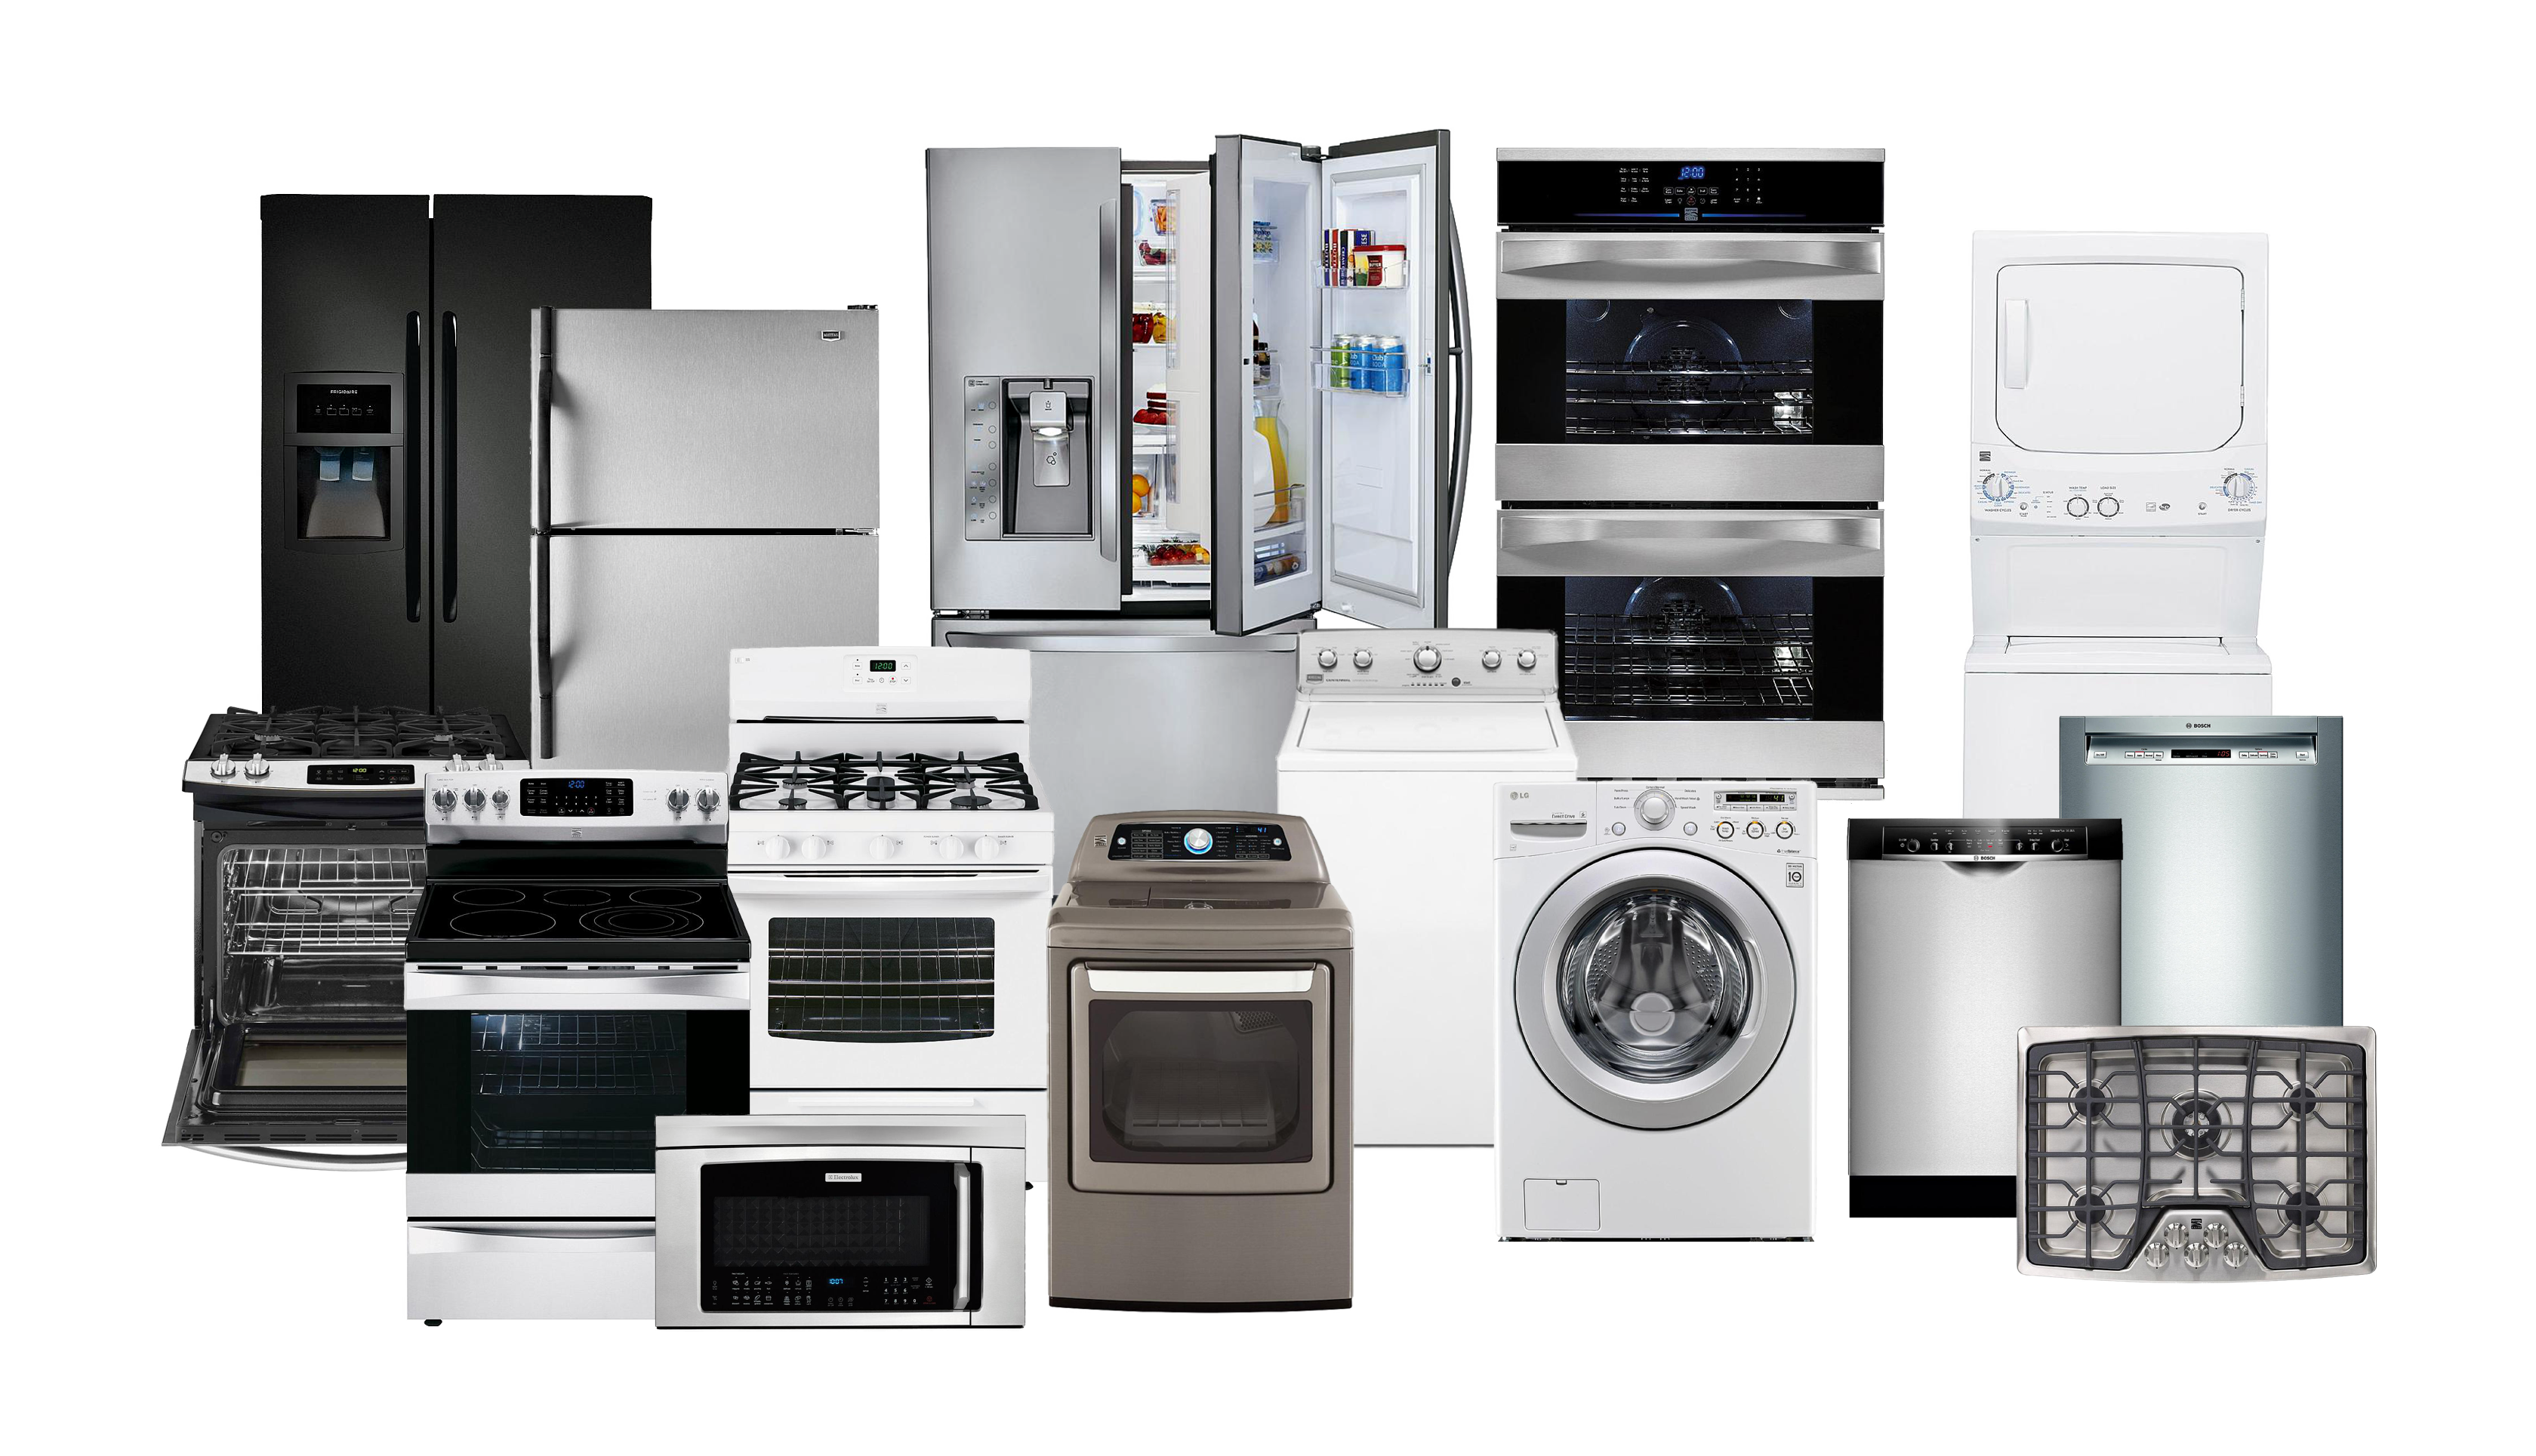
\includegraphics[width=6em]{img/appliances.png} &
			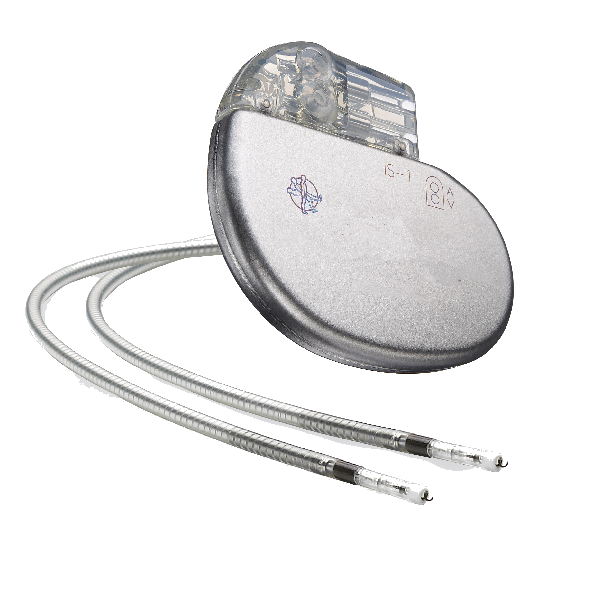
\includegraphics[width=6em]{img/Permanent-Pacemaker.png} &
			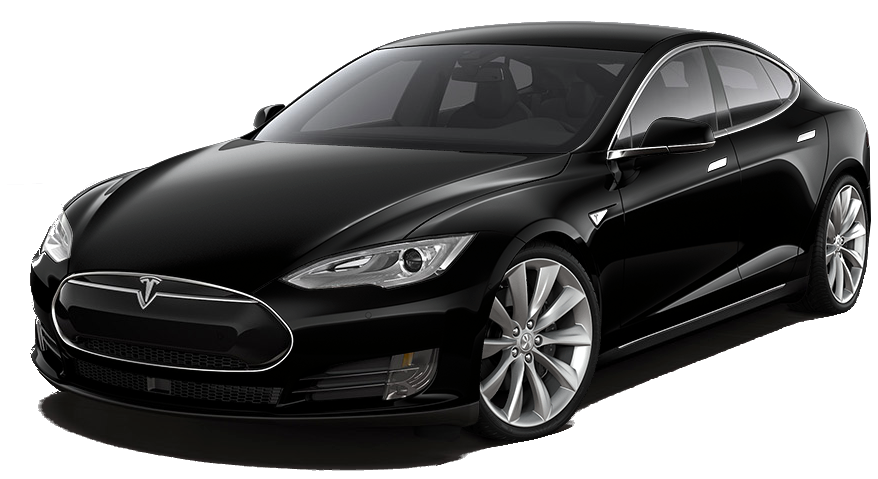
\includegraphics[width=6em]{img/must_diagonaal1.png} \\
			\tiny{Cellphones} &
			\tiny{Appliances} &
			\tiny{Medical Devices} &
			\tiny{Transportation}
		\end{tabular}
	\end{frame}
	
	\begin{frame}{Where Can You Find Embedded Systems?}
		\begin{tabular}{c c c c}		
			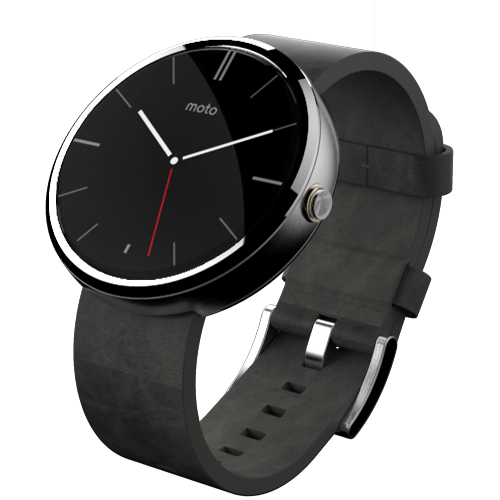
\includegraphics[width=6em]{img/Motorola_Moto_360_Minimal_Watch_Face.png} &
			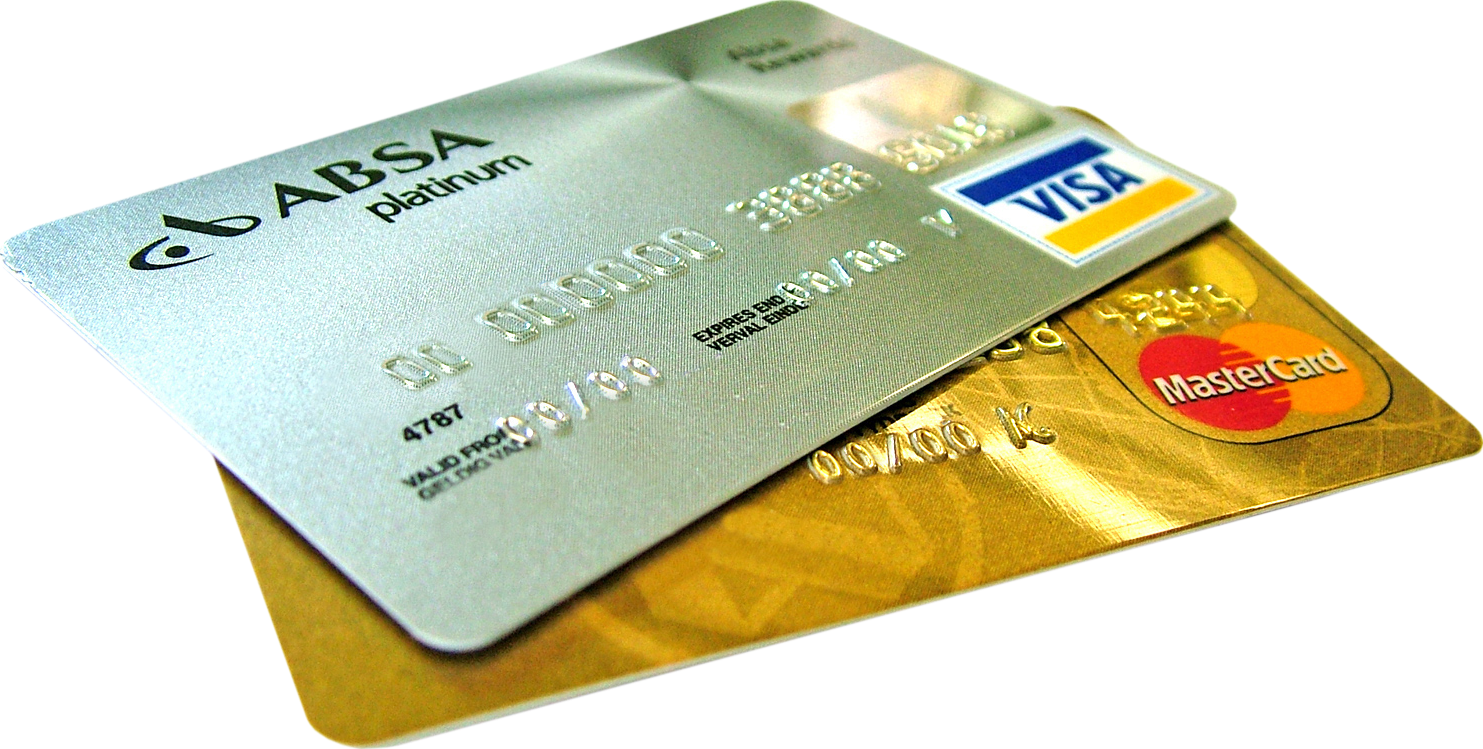
\includegraphics[width=6em]{img/creditcards.png} &
			
\includegraphics[width=6em]{img/IMG_0198} &
			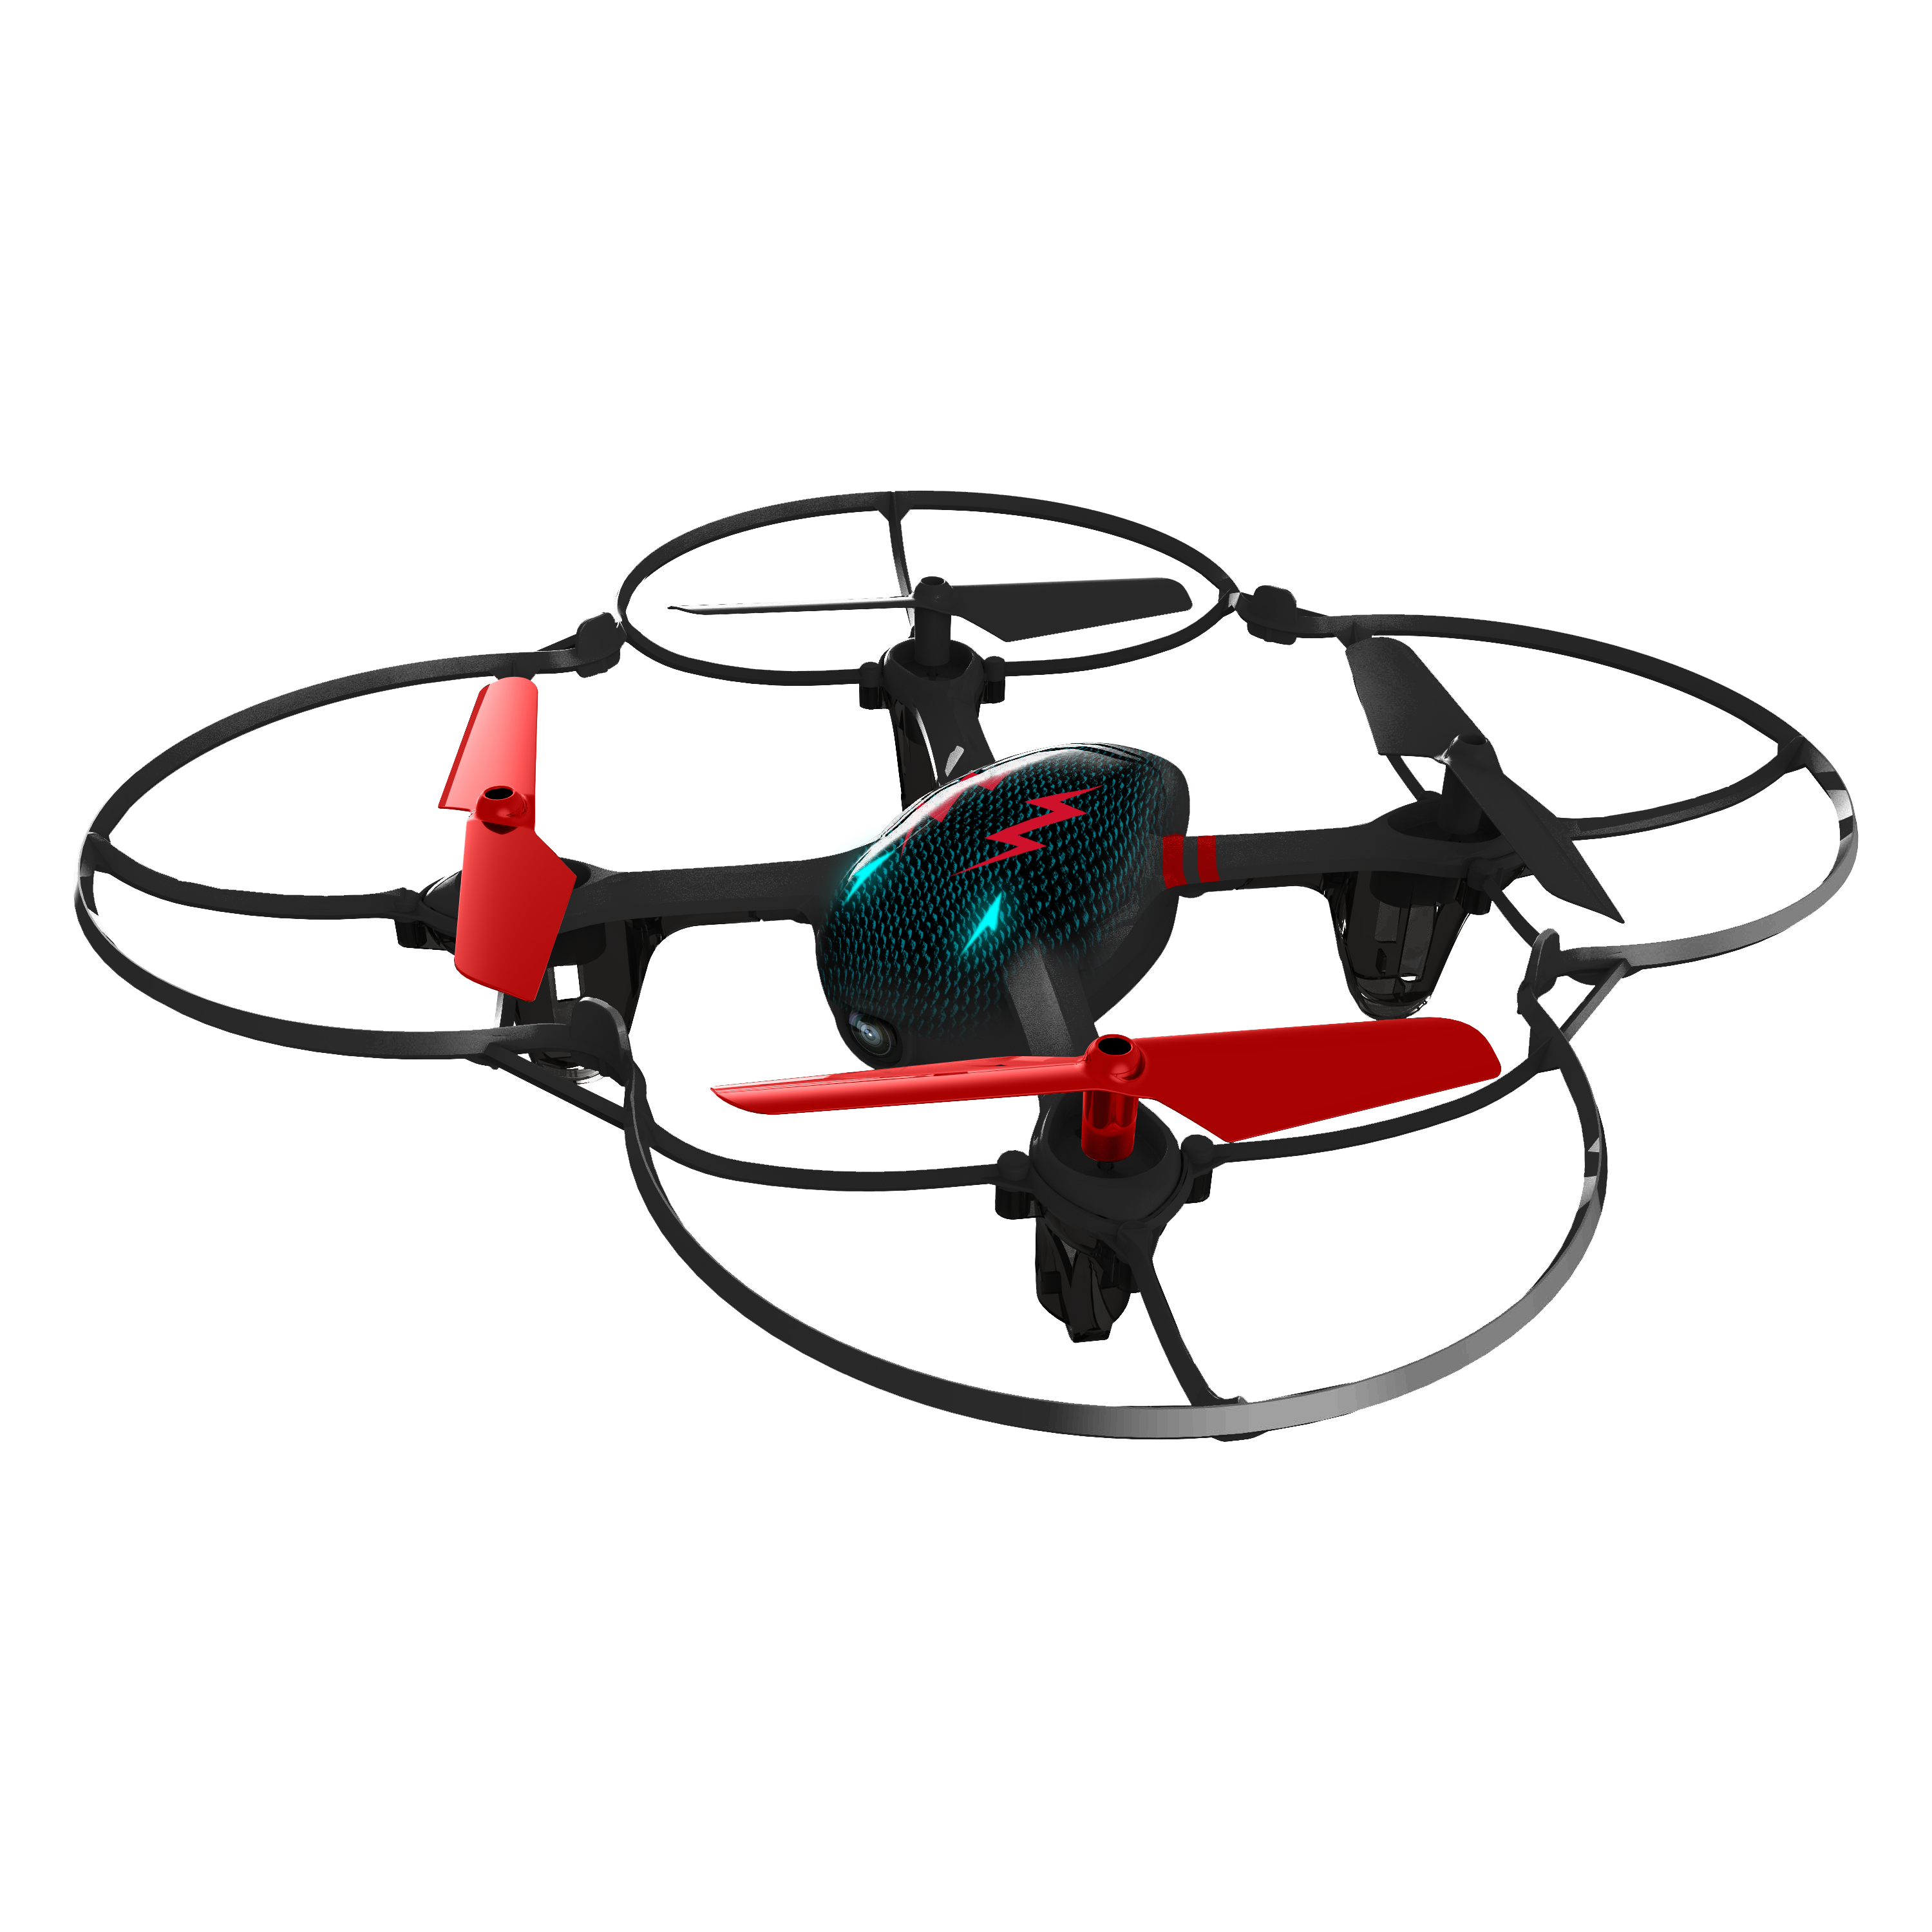
\includegraphics[width=6em]{img/electro_max_eye_720p_video_drone_angle_left} \\
			\tiny{Watches} &
			\tiny{Credit Cards} &
			\tiny{Pets} &
			\tiny{Toys}
		\end{tabular}
		
		\vspace{3em}	
		
		Let's just say that embedded systems are everywhere.
	\end{frame}
  
	% Simple way to visualize an embedded (control) system
	\begin{frame}{Framework For a Simple Embedded (Control) System}
	\begin{center}		
		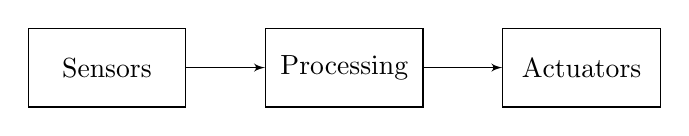
\begin{tikzpicture}[auto, node distance=2cm,>=latex']
			\tikzset{block/.style= {draw, rectangle, align=center,minimum width=2cm,minimum height=1cm},
        rblock/.style={draw, shape=rectangle,rounded corners=1em,align=center,minimum width=2cm,minimum height=1cm},
        input/.style={ % requires library shapes.geometric
        draw,
        trapezium,
        trapezium left angle=60,
        trapezium right angle=120,
        minimum width=2cm,
        align=center,
        minimum height=1cm
    },
        }

			\node [block](sensors) {Sensors};
			\node [block, right=1cm of sensors] (processing) {Processing};
			\node [block, right=1cm of processing] (actuators) {Actuators};
			
			\path[draw,->] (sensors) edge (processing);
			\path[draw,->] (processing) edge (actuators);

		\end{tikzpicture}
	\end{center}	
	\end{frame}
  
  	% Spark control in an ICE
	\begin{frame}{Example: Spark Control in an Internal Combustion Engine}
	
		Problem: We need to generate a spark in the combustion chamber (cylinder) when 
				 the piston is at a particular position.
		
		Complication: The position where we need to create the spark is not a constant!
					  It changes as a function of (primarily) engine speed and engine load.
					  
					  We could get into the whys of this, but this isn't a combustion course.
	
	\end{frame}	  
  
	% distributor cap
	\begin{frame}[t]{Example: Spark Control in an Internal Combustion Engine}
		
		Back in the (dark) days of purely mechanical systems...
			
		\begin{figure}
		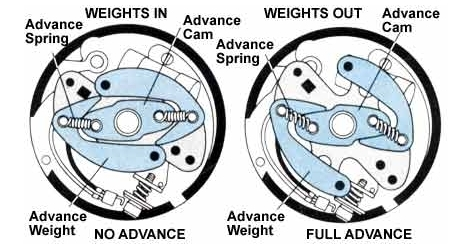
\includegraphics[scale=0.75]{img/3-8-ignition_clip_image005.jpg}
		\caption{http://www.scuderiatopolino.com/3-8-ignition.php}
		\end{figure}
		\href{https://www.youtube.com/watch?v=RcmkbQVPz9E}{Mechanical Spark Advance In Action}
		
	\end{frame}
	
	\begin{frame}{Example: Spark Control in an Internal Combustion Engine}
	
		Today, we use a simple embedded control system: 
				
		{\bf Inputs (Sensors):}
		\begin{itemize}
			\item Crankshaft position
			\item Crankshaft speed
			\item Throttle position
		\end{itemize}
		
		{\bf Processing:}
		\begin{itemize}
			\item A 2-D lookup table of spark time vs. \\
			engine speed and throttle position
		\end{itemize}
		
		{\bf Outputs (Actuators):}
		\begin{itemize}
			\item Signal to close spark contact
		\end{itemize}
	
	\end{frame}
	
	\begin{frame}{Inside a Smartphone}
		
		Since we're going to be using Android in this course, let's take a brief look
		inside my favourite phone, the {\bf OnePlus One}.
		
		\href{https://www.ifixit.com/Teardown/OnePlus+One+Teardown/26484}{https://www.ifixit.com/Teardown/OnePlus+One+Teardown/26484}
		
		\vspace{1em}		
		
		\centering
		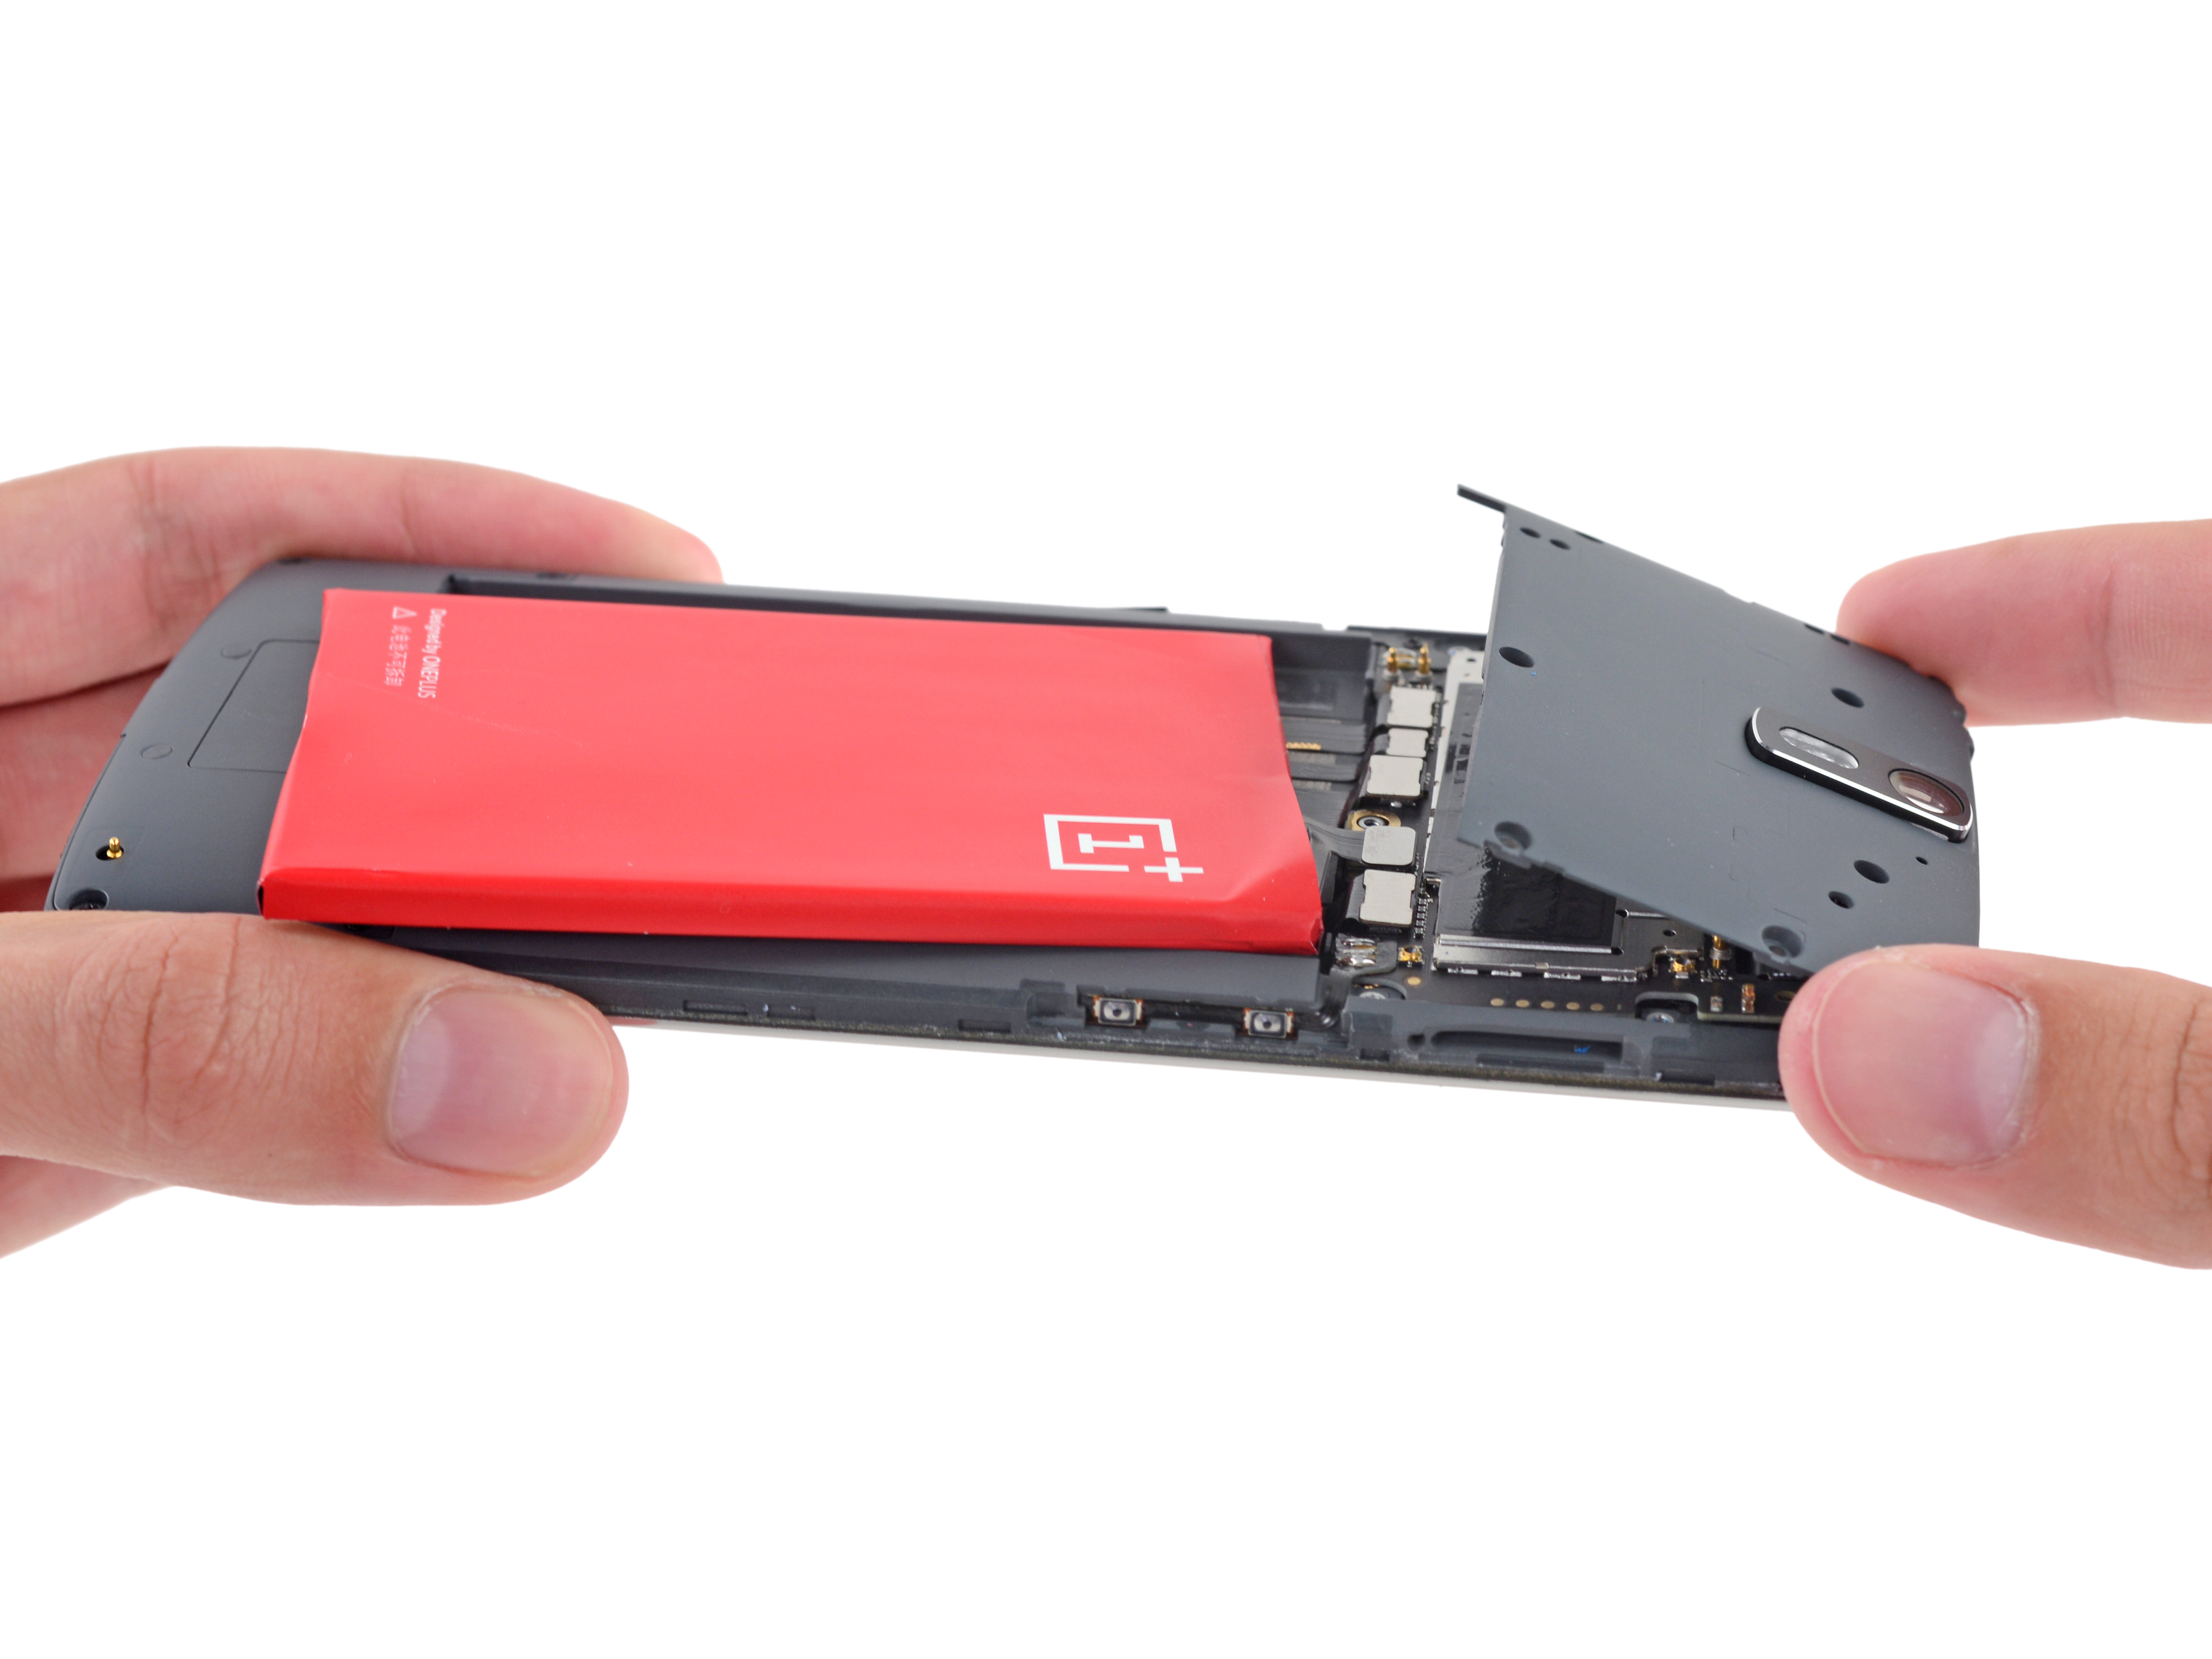
\includegraphics[width=\textwidth,height=6cm,keepaspectratio]{img/WJweKyYej2qtrc4m.png}
			
	\end{frame}
	
	\begin{frame}{Inside a Smartphone}
		We have two cameras (sensors) sitting at the top of the phone.
		\begin{figure}[b]		
		\centering
		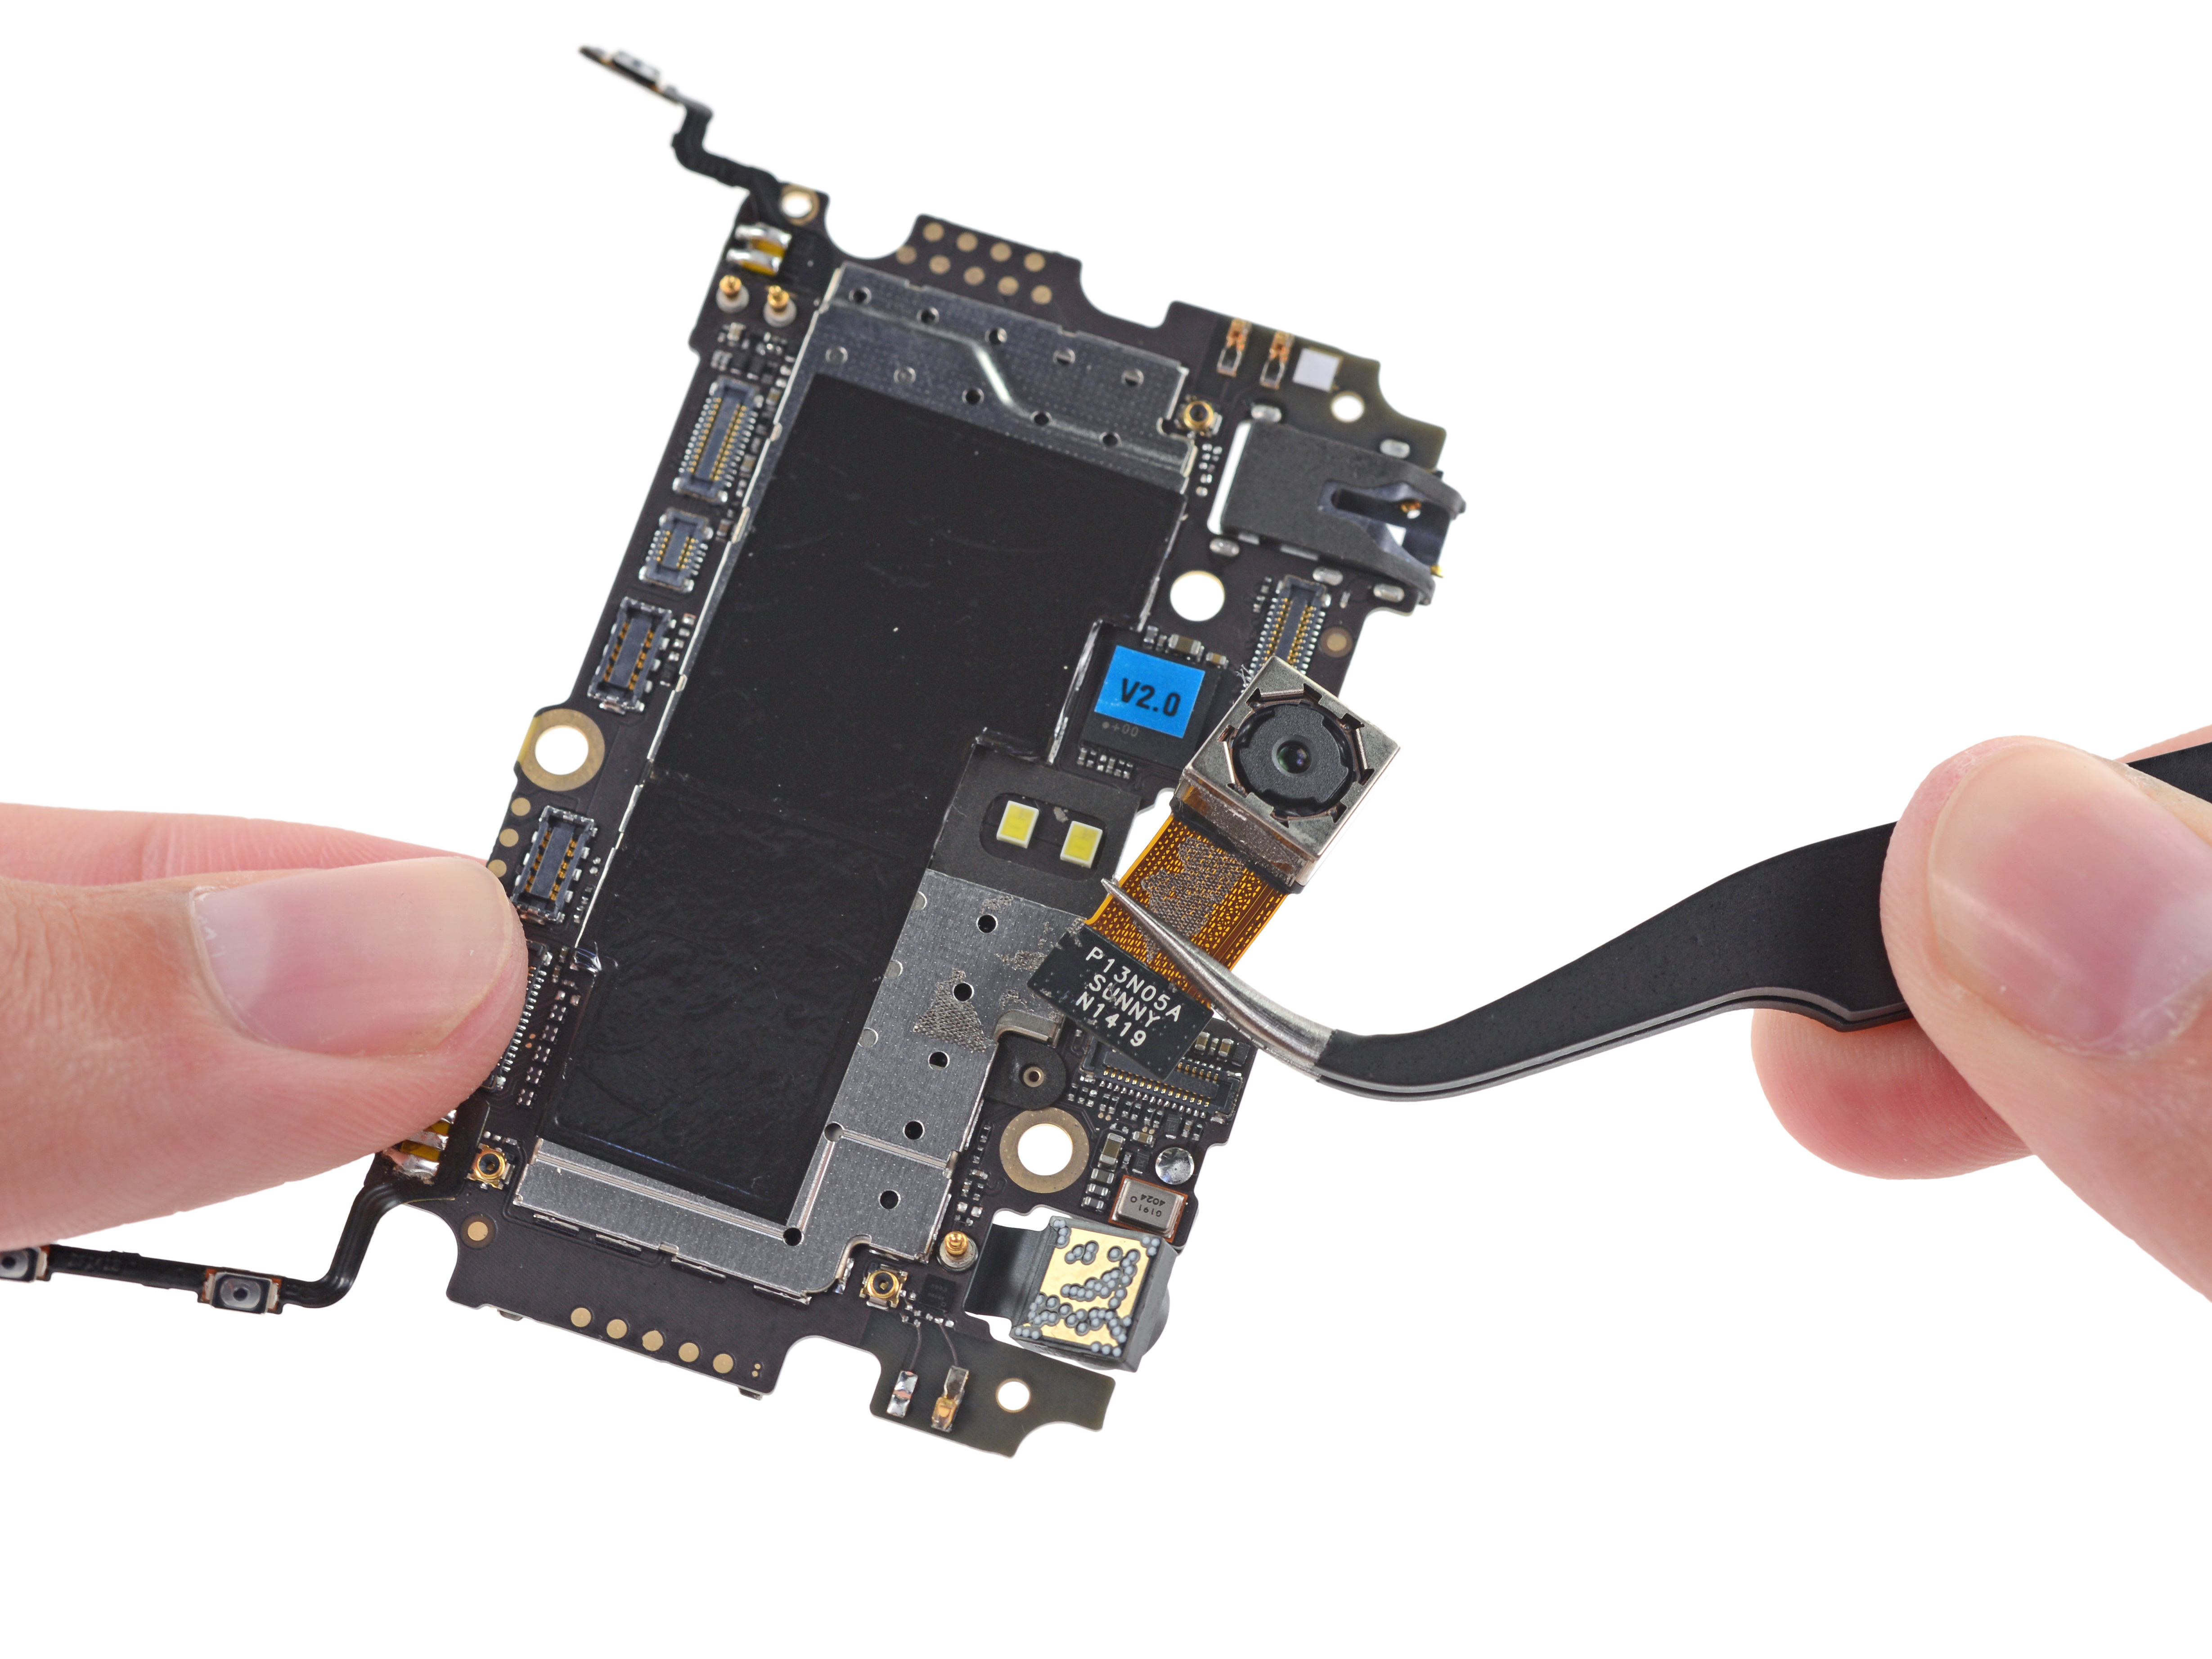
\includegraphics[width=\textwidth,height=6cm,keepaspectratio]{img/SuhLygXH4QXdDMEm.png}
		\end{figure}
	\end{frame}
  
	\begin{frame}{Inside a Smartphone}
		The motherboard is crammed full of embedded components...
		\begin{figure}[b]
		\centering
		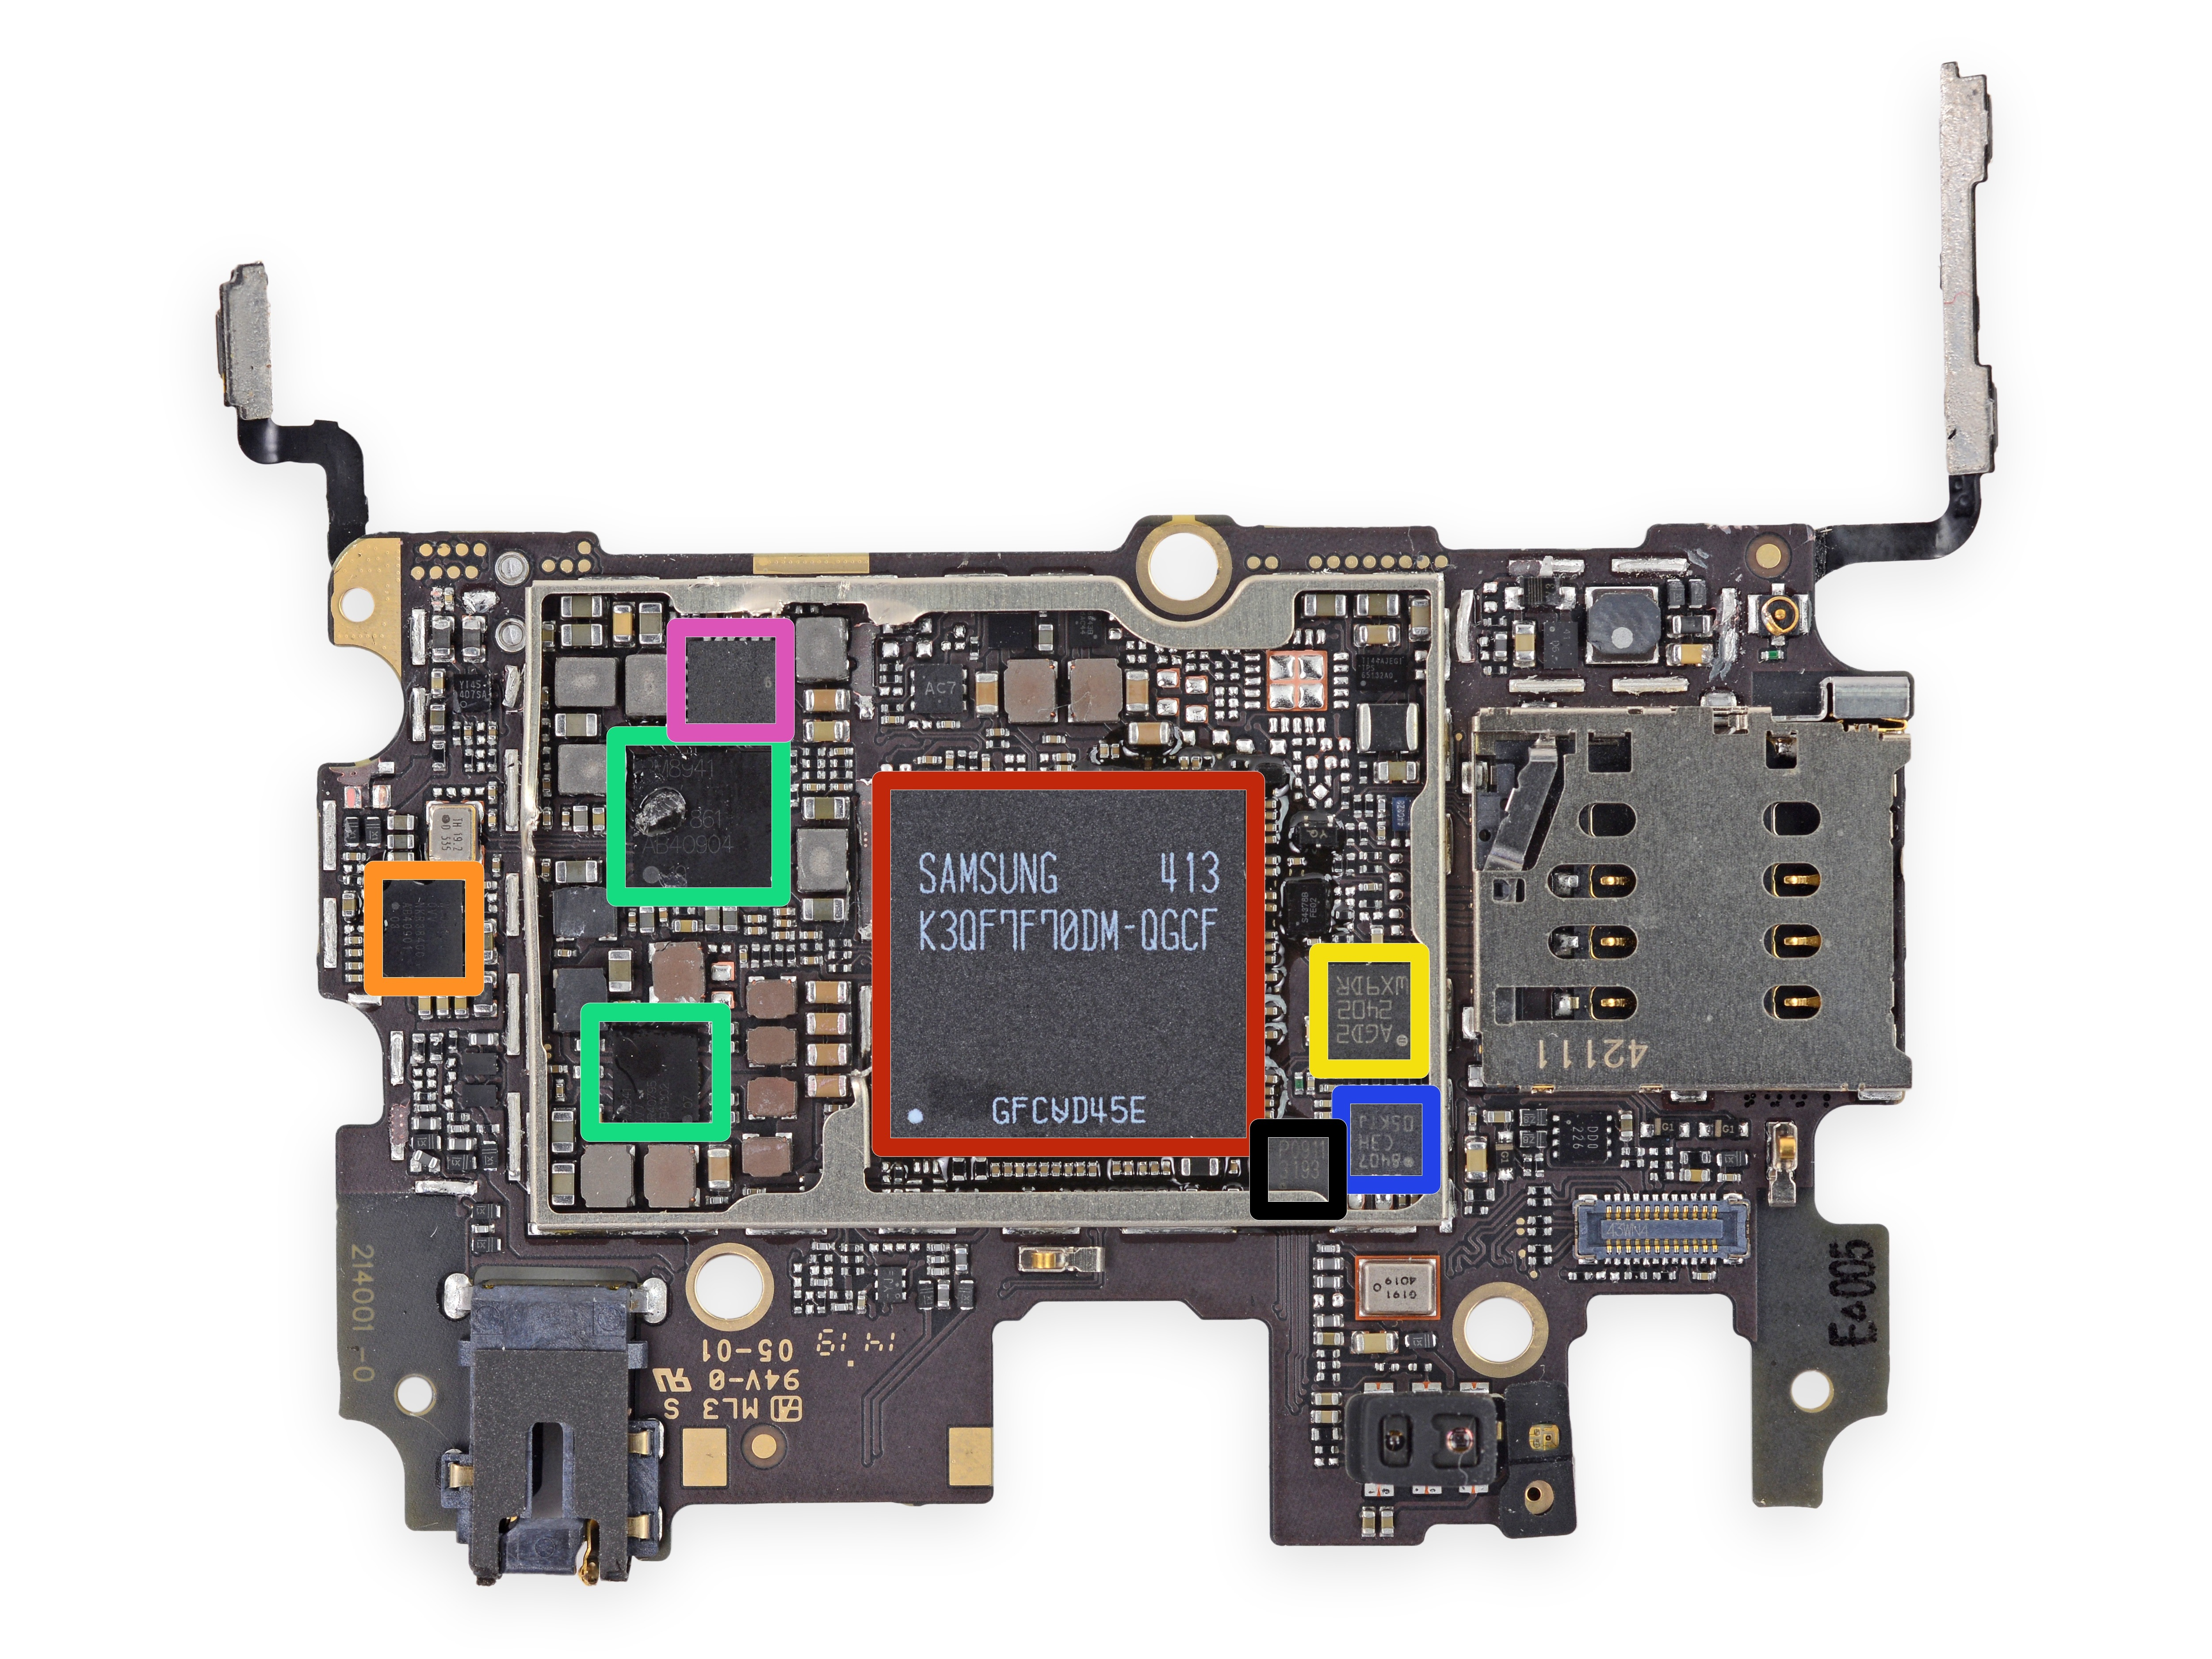
\includegraphics[width=\textwidth,height=6cm,keepaspectratio]{img/wIp5pQj4movpelpR.png}
		\end{figure}
	\end{frame}  
	
	\begin{frame}{Inside a Smartphone}
		...on both sides
		\begin{figure}[b]
		\centering
		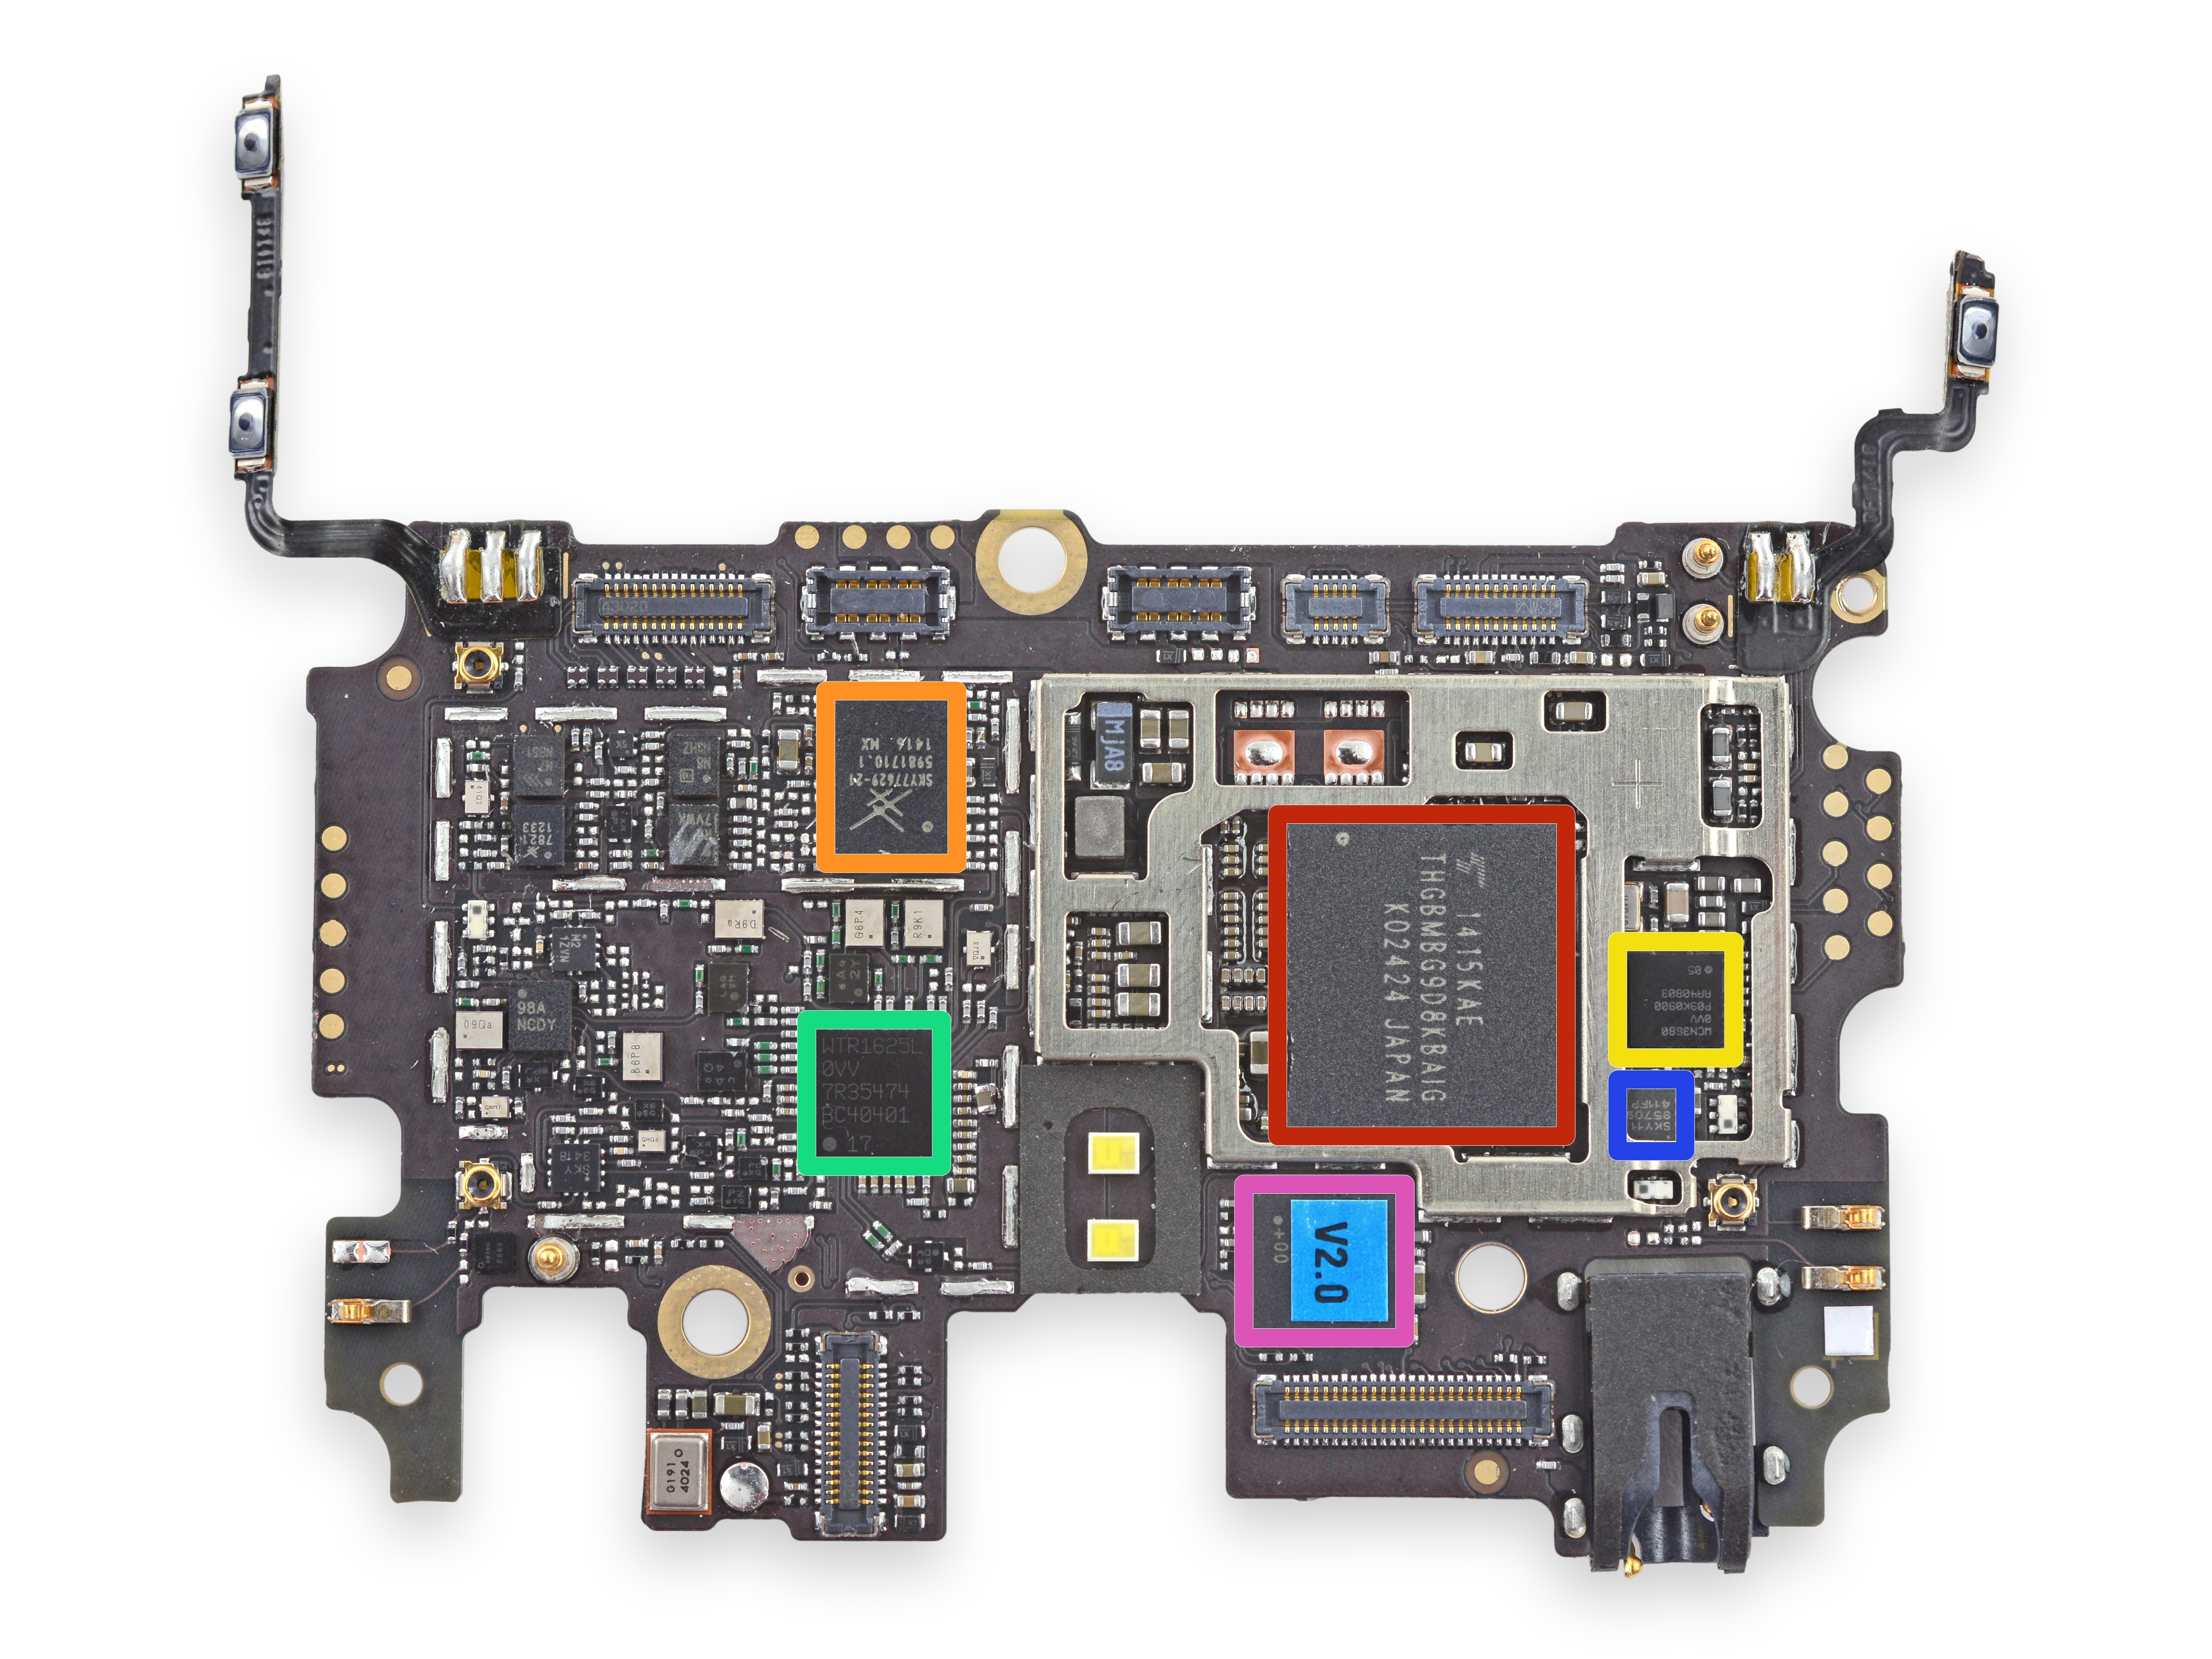
\includegraphics[width=\textwidth,height=6cm,keepaspectratio]{img/FGcUA3hpq1ejhOQL.png}
		\end{figure}
	\end{frame}
  
	\begin{frame}{Inside a Smartphone}
		The daughter-board at the bottom contains some actuators.
		\begin{figure}[b]
		\centering
		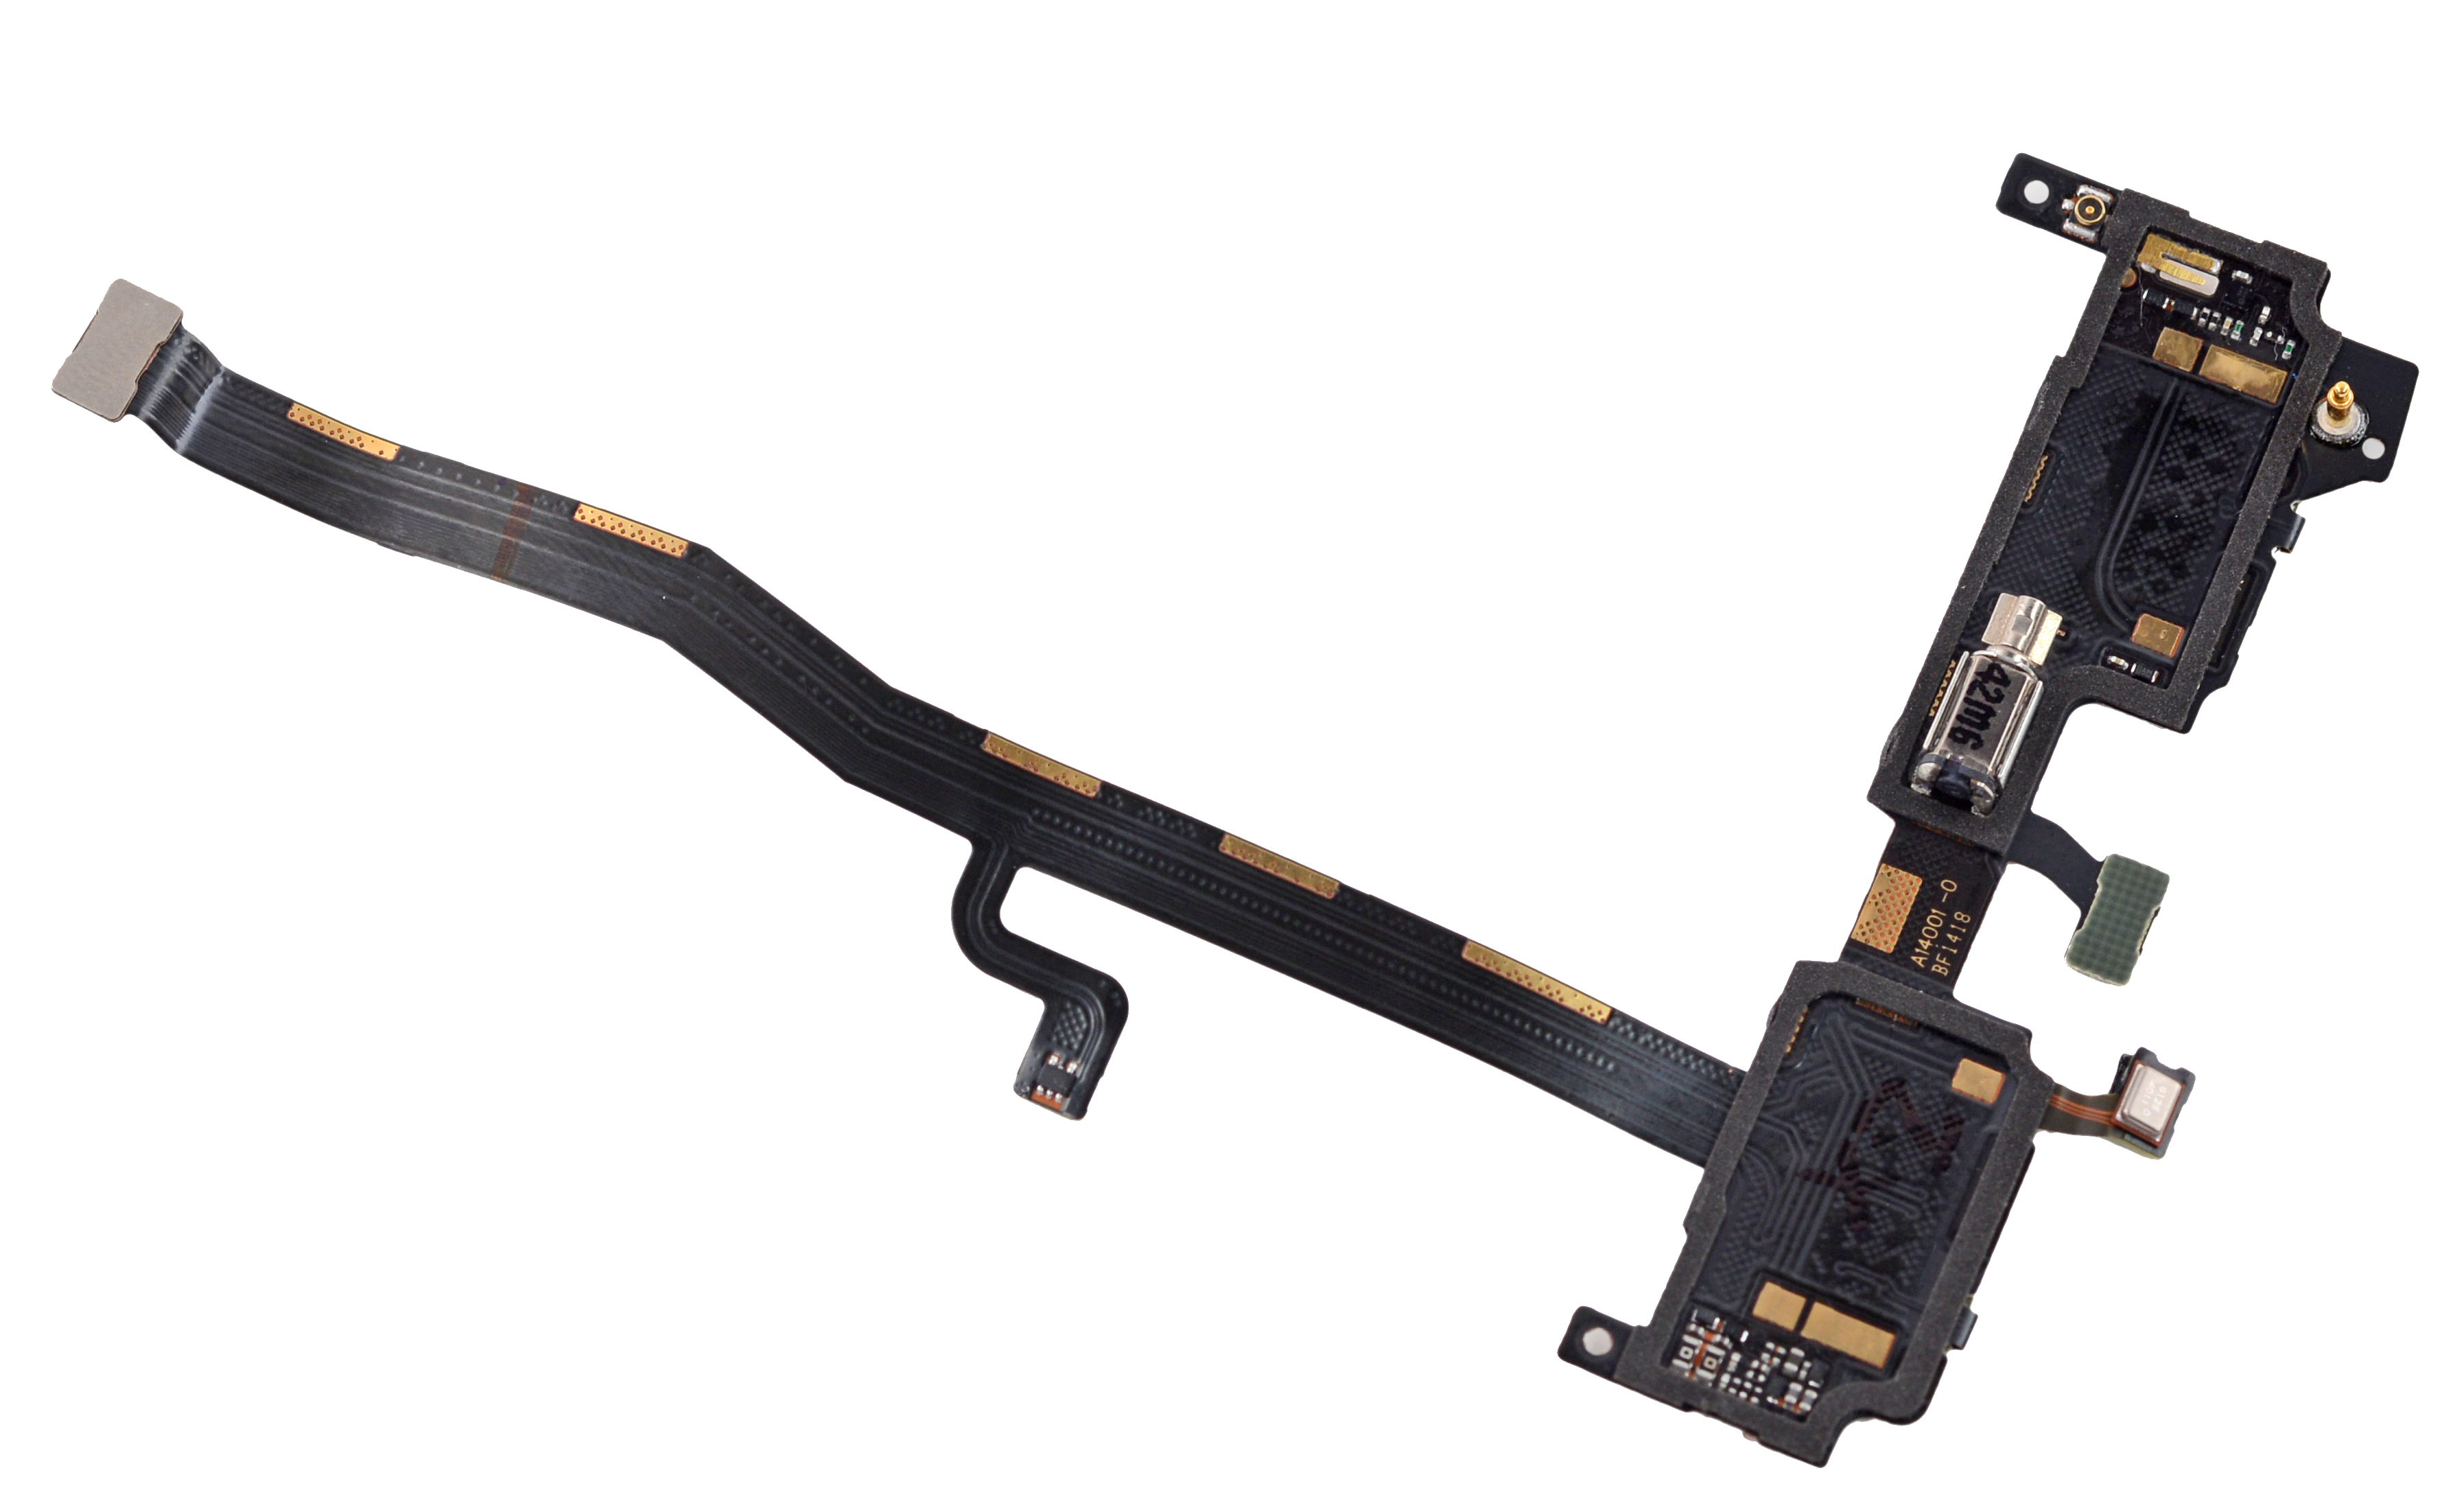
\includegraphics[width=\textwidth,height=6cm,keepaspectratio]{img/wdnGHA1UB3lBpZIL.png}
		\end{figure}
	\end{frame}    
	
	\begin{frame}[t]{About Sensors}
		\small Sensors measure real-world phenomena and convert them into signals that we can process.	\\
		\vspace{0.5em}
		\begin{figure}
			\centering
			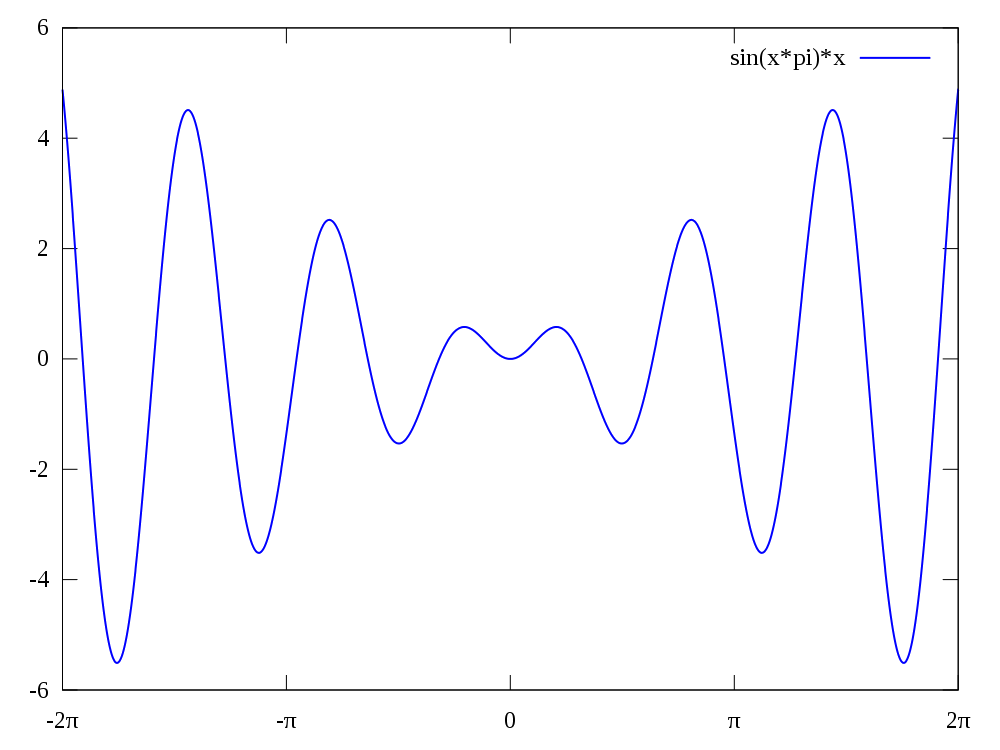
\includegraphics[width=\textwidth,height=0.6\textheight,keepaspectratio]{img/sine.png}
		\end{figure}
		Sensor results (in Volts, say) are continuous and analog...	\\	
		\hspace{2em}...but computers are discrete-time and digital. \\	
		\vspace{2em}		
		What to do? \\
	\end{frame}
	
\begin{frame}[fragile]{About Sensors}
\small{To convert an analog signal (e.g. voltage) to a digital value, we use an {\bf Analog-To-Digital Converter (ADC).}}	\\
\vspace{0.5em}
\begin{figure}[b]
\centering
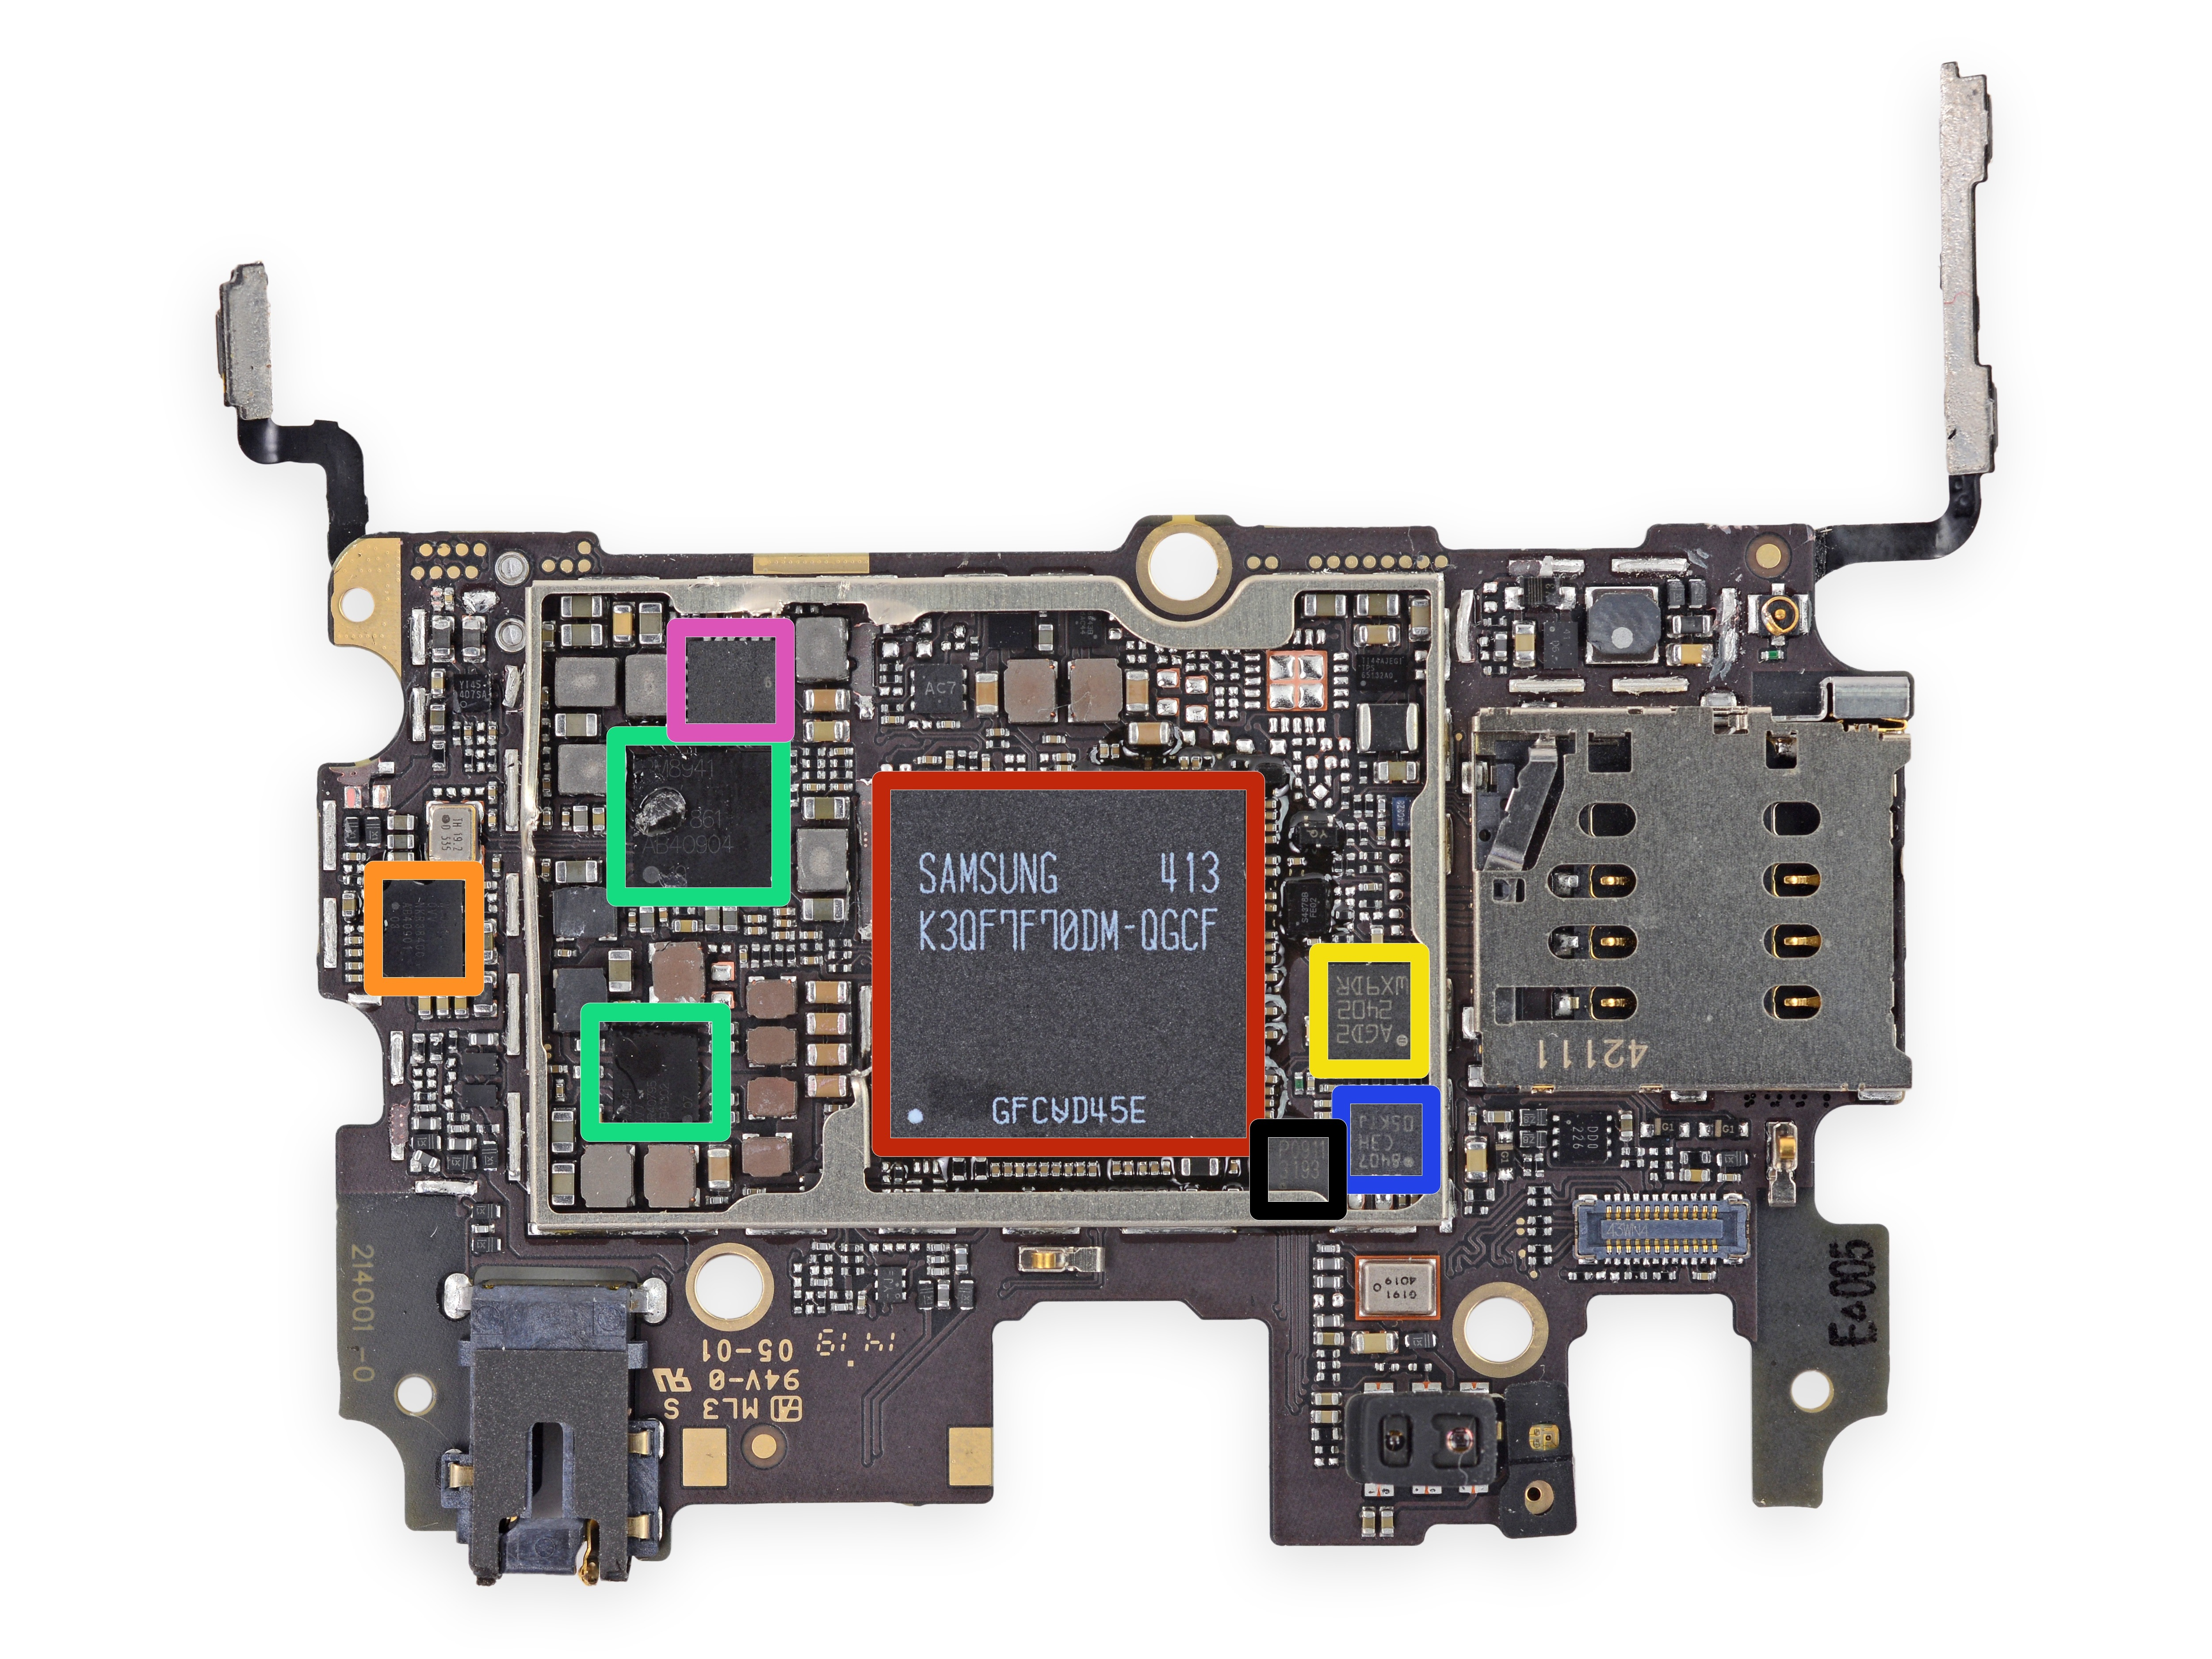
\includegraphics[width=\textwidth,height=6cm,keepaspectratio]{img/wIp5pQj4movpelpR.png}
\end{figure}
\end{frame}	
	
\begin{frame}[fragile]{About Sensors}
\small To handle a continuous-time signal, we "sample" the signal at discrete times.	\\
\vspace{0.5em}
\begin{tabular}{@{}m{0.6\textwidth} m{0.4\textwidth}@{}}
\begin{figure}
\centering
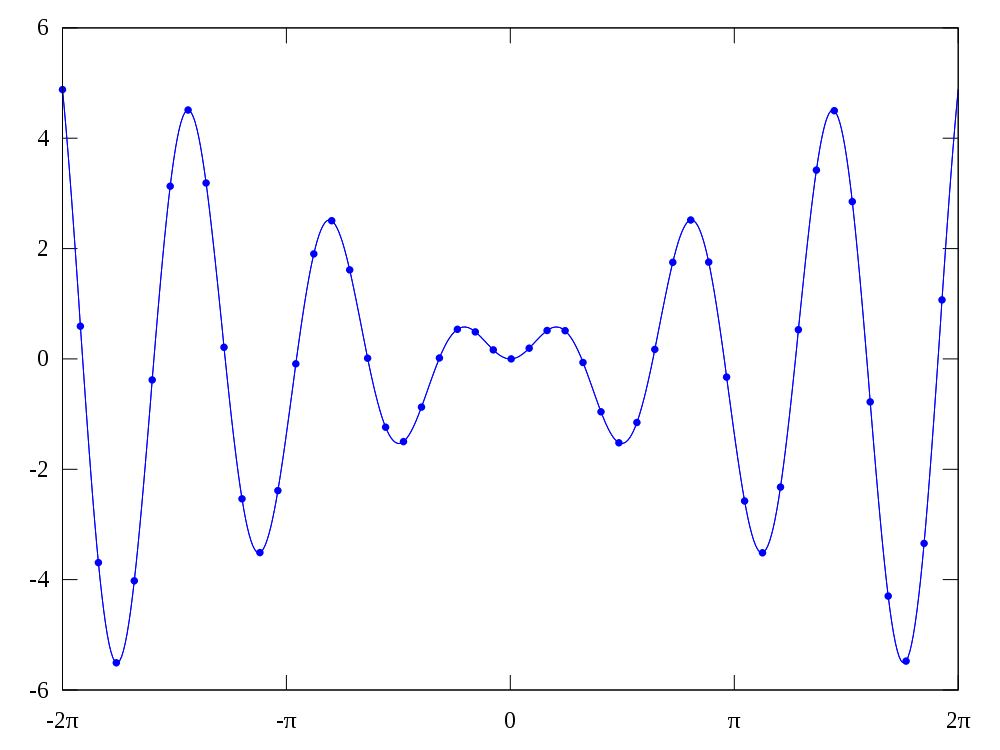
\includegraphics[width=0.6\textwidth,height=0.6\textheight,keepaspectratio]{img/sine-points.png}
\end{figure}
&
\begin{Verbatim}[fontsize=\scriptsize]
while(true)
{
  int y = sensor.read();
  int x = now();
  sleep(0.2);
}		
\end{Verbatim}	
\end{tabular}
\vspace{0.5em}
e.g. (0, 0), (0.2, 0.12), (0.4, 0.38), (0.6, 0.57), (0.8, 0.47)	\\	
\end{frame}
  
\begin{frame}{ADC Output}
We lose information if samples too infrequent\footnote{Nyquist sampling theorem.}, or if sample resolution too poor.
\begin{center}
\begin{tabular}{r|r}
Time (ms) & Signal (V) \\ \hline
0.0 & 0.00 \\
0.2 & 0.12 \\
0.4 & 0.38 \\
0.6 & 0.57 \\
0.8 & 0.47 \\
\end{tabular}
\end{center}
~\\[1em]
How would we increase sample frequency? Sample resolution?
\end{frame}  
 
\begin{frame}{About Actuators}
Actuators take signals from our embedded system and convert them into physical phenomena. \\
\vspace{5em}
What if our actuator requires an analog signal? We use a {\bf Digital-to-Analog Converter (DAC)}.
\end{frame}  
  
\begin{frame}[t]{Processing}
\small
Embedded systems cover a wide range of complexity, and it's common to have multiple systems working together. \\
\vspace{1em}
\begin{figure}
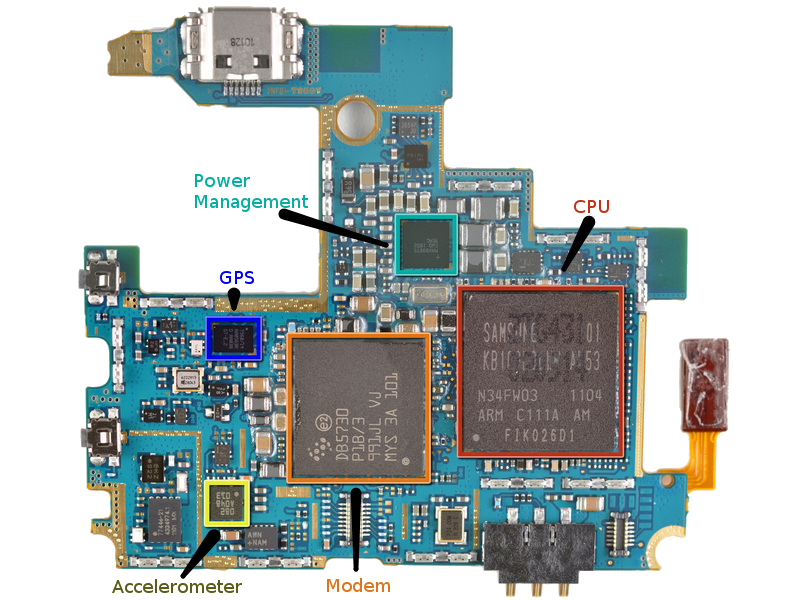
\includegraphics[width=\textwidth,height=0.6\textheight,keepaspectratio,left]{img/Galaxy_Logic_Board_Edited_2_small_annotated.png}
\captionsetup{justification=raggedright,singlelinecheck=false,labelformat=empty}
\caption{Samsung Galaxy S motherboard}
\end{figure}
\end{frame}  

\begin{frame}[t]{Processing}
\small
Embedded systems cover a wide range of complexity, and it's common to have multiple systems working together. \\
\vspace{1em}
\begin{figure}
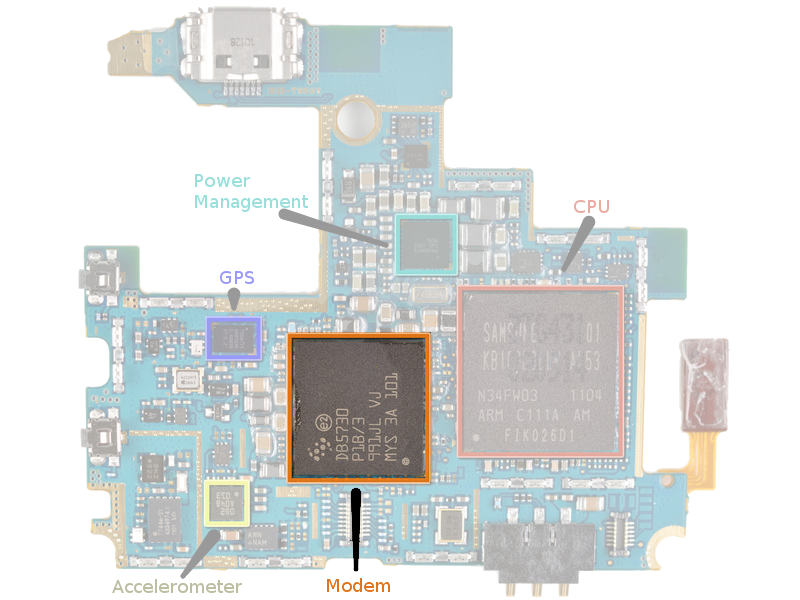
\includegraphics[width=\textwidth,height=0.6\textheight,keepaspectratio,left]{img/Galaxy_Logic_Board_Edited_2_small_annotated_highlight_modem.png}
\captionsetup{justification=raggedright,singlelinecheck=false,labelformat=empty}
\caption{Samsung Galaxy S motherboard}
\end{figure}
\end{frame} 

\begin{frame}[t]{Processing}
\small
Embedded systems cover a wide range of complexity, and it's common to have multiple systems working together. \\
\vspace{1em}
\begin{figure}
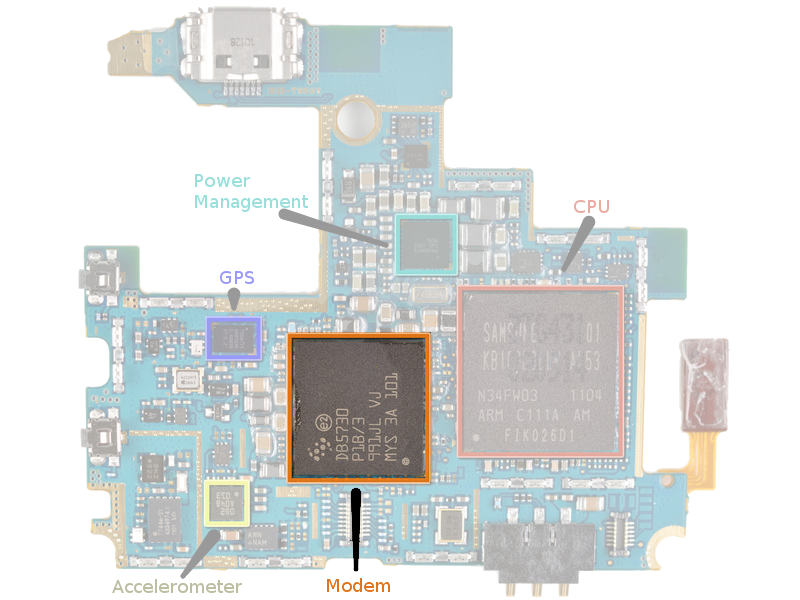
\includegraphics[width=\textwidth,height=0.6\textheight,keepaspectratio,left]{img/Galaxy_Logic_Board_Edited_2_small_annotated_highlight_modem.png}
\captionsetup{justification=raggedright,singlelinecheck=false,labelformat=empty}
\caption{Samsung Galaxy S motherboard}
\end{figure}
\putat{110}{95}{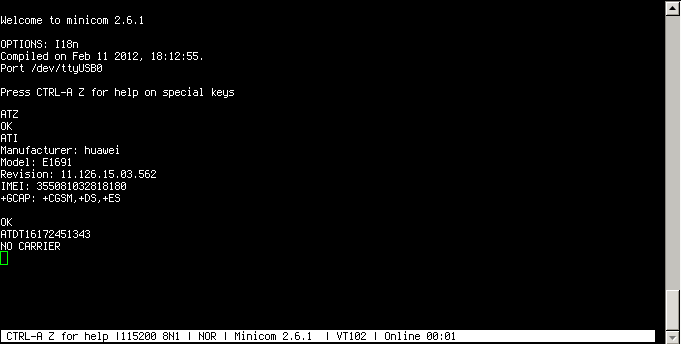
\includegraphics[scale=0.32]{img/modem-interaction.png}}
\end{frame} 

\begin{frame}
\frametitle{Running an Embedded Control Program}

The modem is running an \alert{embedded control program}.
\begin{itemize}
\item accepts high-level commands from the CPU;
\item translates bits into analog signals; contains ADC and DAC.
\end{itemize}

\vspace{1em}More generally, the modem:
\begin{itemize}
\item boots automatically,
\item never terminates,
\item translates stream of sensor inputs and actuator outputs,
\item cares about timing.
\end{itemize}
\end{frame}

\begin{frame}{What about the OnePlus One?}
Where's the modem in the OnePlus One? \\
\begin{figure}[b]
\centering
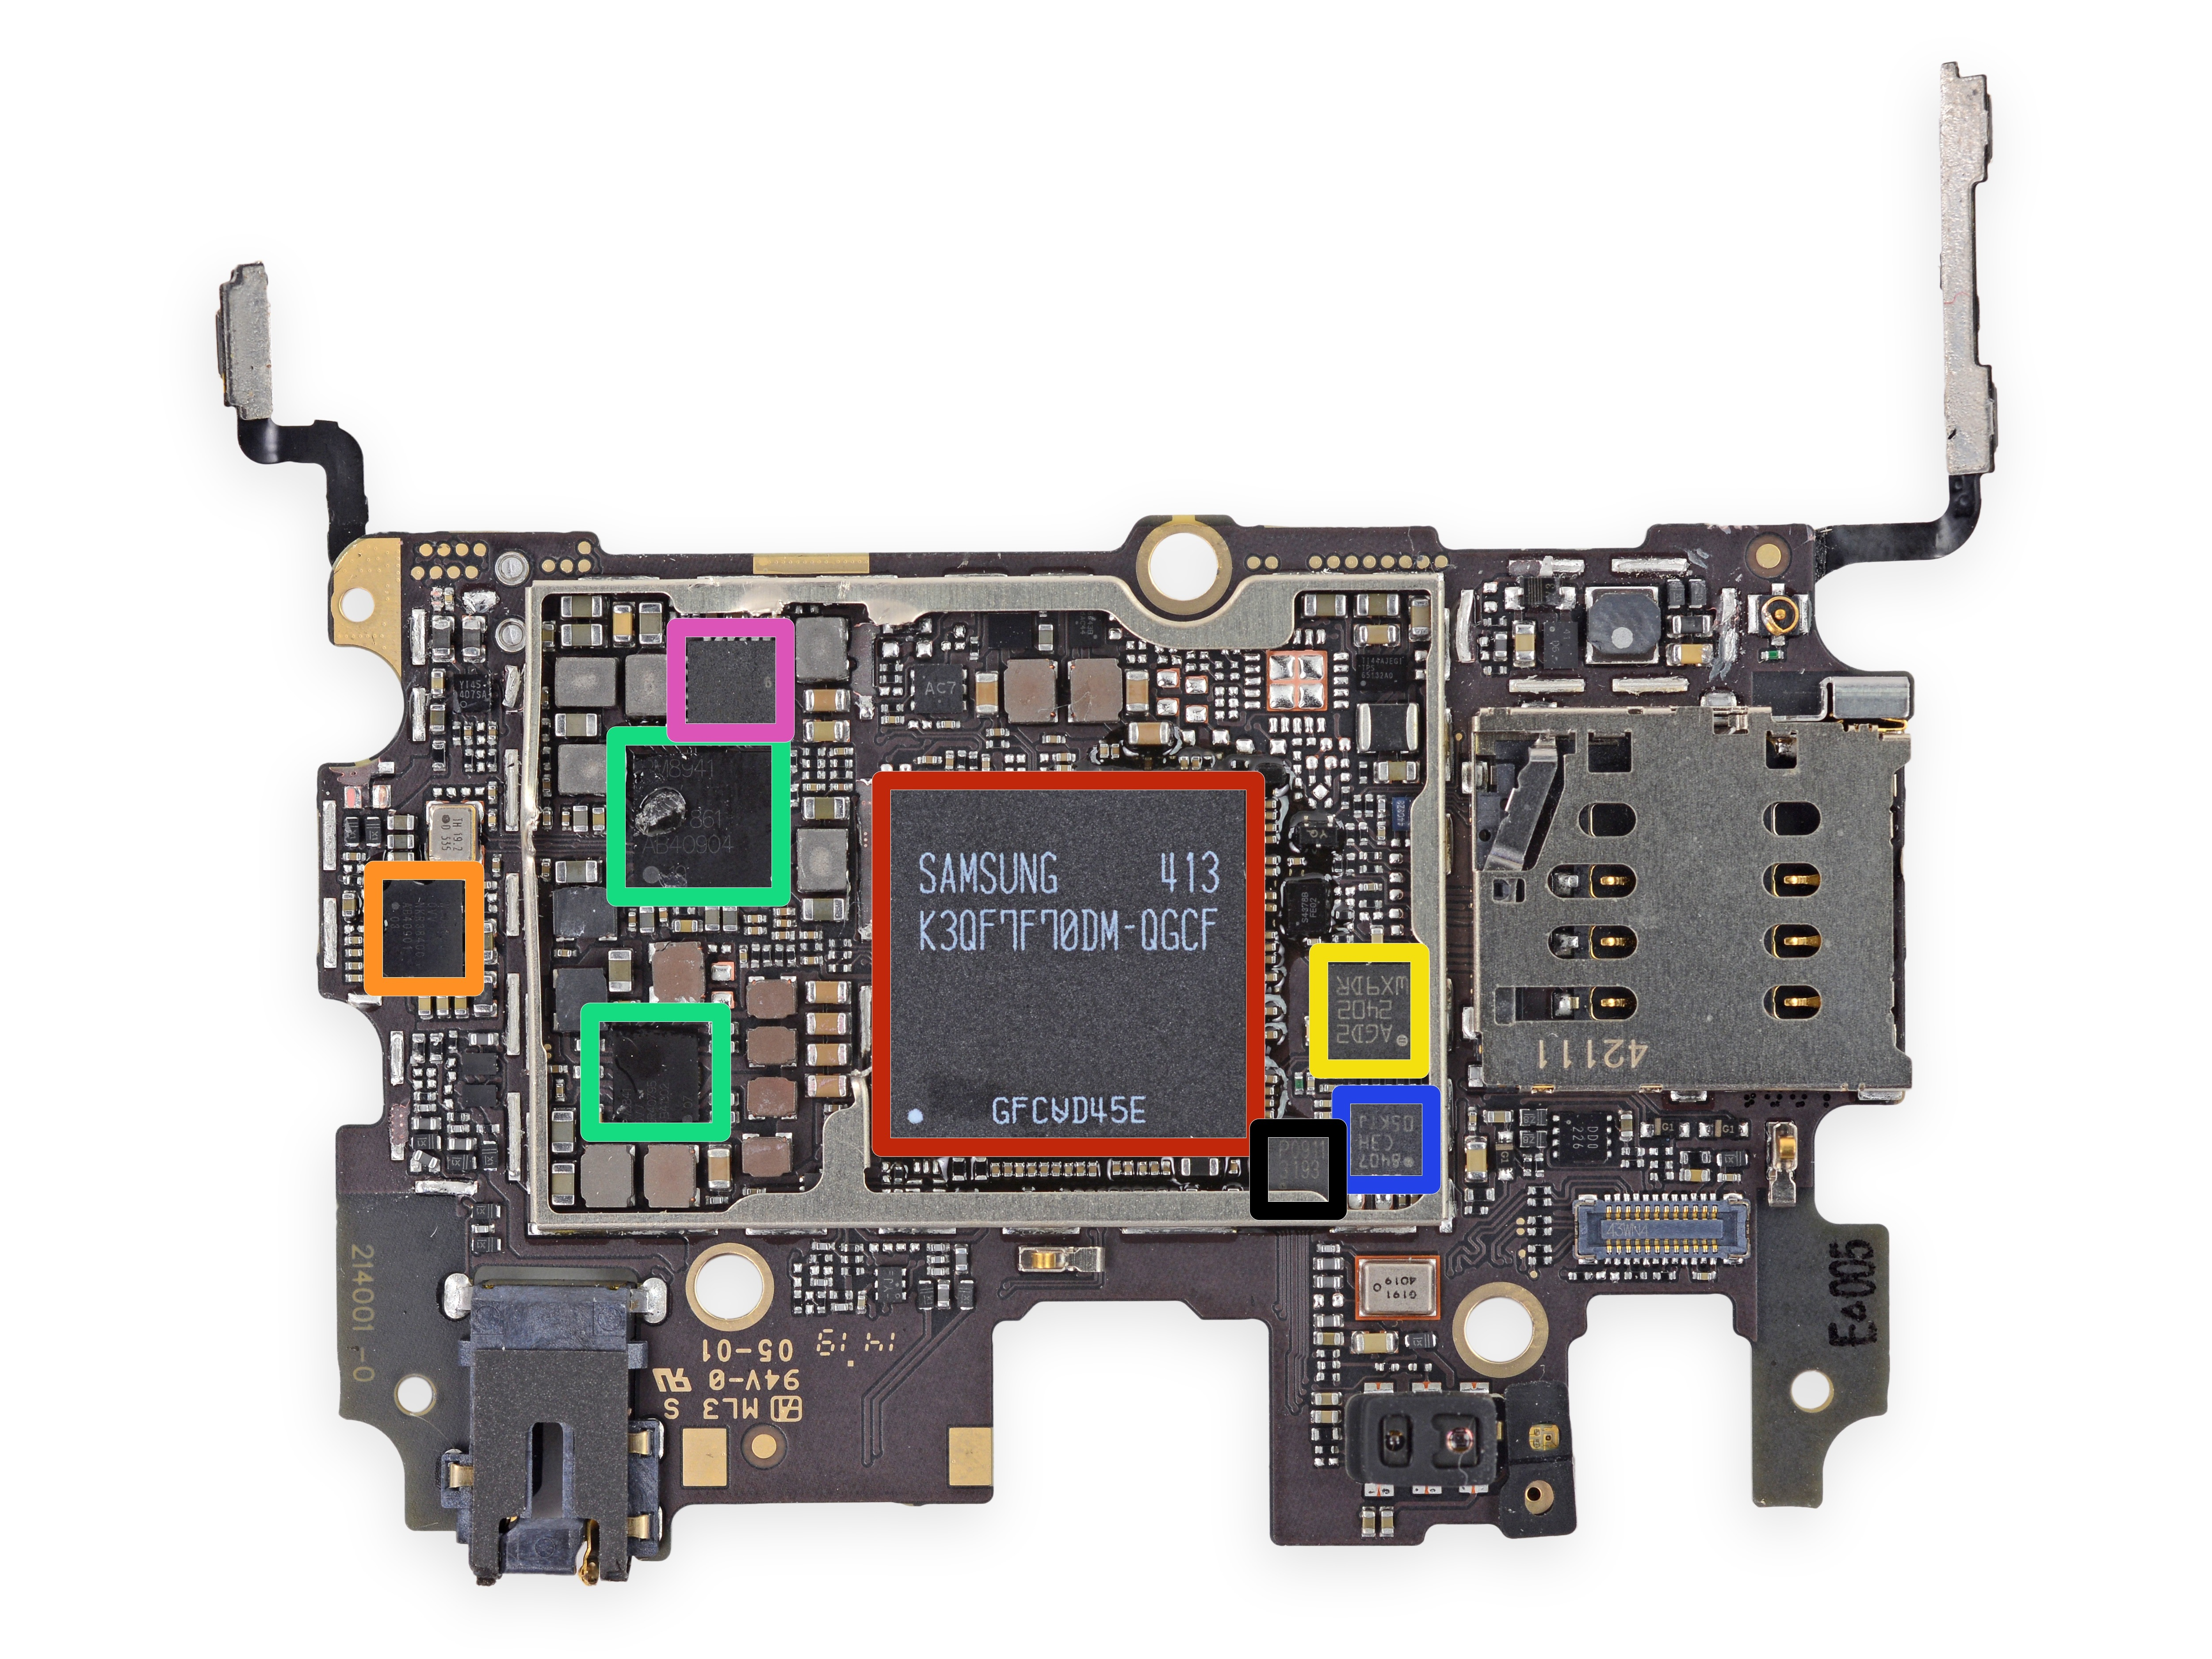
\includegraphics[width=\textwidth,height=6cm,keepaspectratio]{img/wIp5pQj4movpelpR.png}
\end{figure}
\end{frame}

\begin{frame}{What about the OnePlus One?}
Where's the modem in the OnePlus One? \\
\begin{figure}[b]
\centering
\includegraphics[width=\textwidth,height=6cm,keepaspectratio]{img/wIp5pQj4movpelpR_snappy.png}
\end{figure}
\end{frame}

\begin{frame}{What about the OnePlus One?}
\begin{figure}[b]
\centering
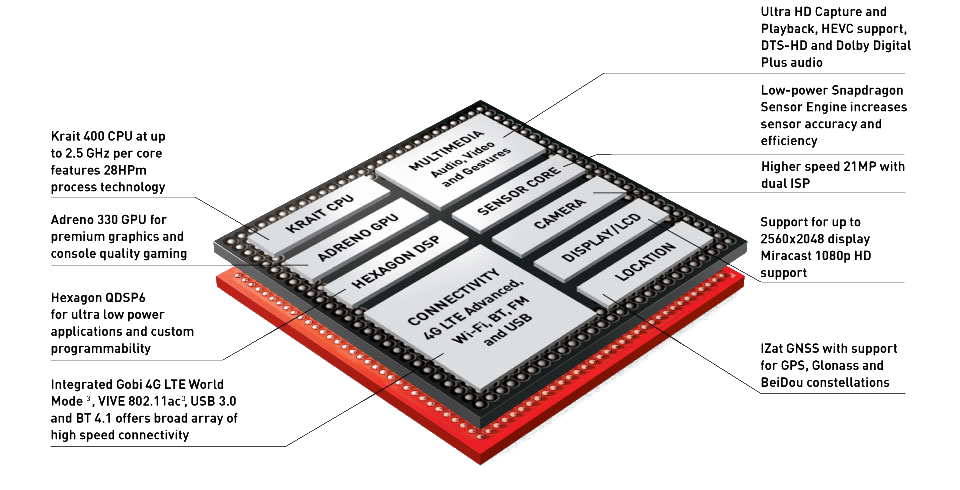
\includegraphics[width=\textwidth,height=6cm,keepaspectratio]{img/snapdragon-801-soc-image.png}
\captionsetup{labelformat=empty,font=scriptsize}
\caption{http://media.bestofmicro.com/V/9/427509/original/snapdragon-801-soc-image.png}
\end{figure}
\end{frame}

\begin{frame}{Embedded Systems and Safety: Therac-25}
\centering
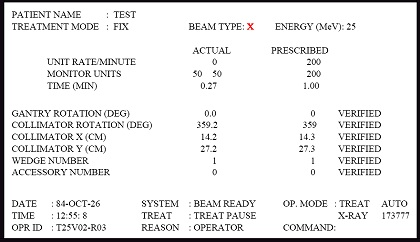
\includegraphics[width=0.8\linewidth]{img/Xraybad.jpg}
\end{frame} 

\begin{frame}{Embedded Systems and Safety: Therac-25}
  \begin{itemize}
  \item Radiation therapy machine
  \item Problem: \alert{many} $\rightarrow$ race conditions, overflow,
    no safety interlocks
  \item 3 patients died!
  \item Fix: software updates
  \end{itemize}

  \note[item]{\textbf{Problem Race Condition:} Race condition between
    the operator interface task ad the equipment control
    task. Occurred only during quick controlling \textbf{(operator
      practice)}.}

  \note[item]{\textbf{Problem Overflow:} flag was incremented,
    overflow caused software to bypass safety checks.}

  \note[item]{\textbf{Problem Interlocks:} high-energy mode was
    enabled without target in place.}
\end{frame}

\begin{frame}[c]
  \frametitle{Conclusion}
  \textbf{\Large Someone has to build these systems!} \\
  Your life will depend on them.

  \pause

   \vspace{2em}
   Chances to learn about building safety-critical systems: \\
   \begin{itemize}
   \item ECE455 Embedded Software
   \item SE499: Independent project
   \item FYDP
   \item Undergraduate research assistant
   \end{itemize}
\end{frame}

\end{document}